% ===========================================================================
%  IntroAct-TS —— ICLR 2027 投稿正文
% ---------------------------------------------------------------------------
%  版本      : v4.4（2026-09-17 首版）
%  模板      : 用户提供的 ICLR 2027 style files（未作任何改动）
%  上一版    : 无（v4.3.1-r5 只有 Markdown 草稿，本文件是第一个 LaTeX 正文）
%
%  重要约定
%  ---------
%  1. 所有尚未在服务器上跑出的数字，一律写成占位符 \ph{KEY}，渲染为灰色
%     [KEY]。绝不允许用估计值、旧协议值或"看起来合理"的数填充。
%     占位符命名规范见 latex/README.md。
%  2. 只有 v4.3.1-r5 台账里已经独立审核过的历史数字，才允许以真实数值出现在
%     Appendix G，并且必须显式标注其属于旧协议、不得与 v4.4 主表比较。
%  3. 正文只保留 4.1-4.6 六个小节，效率并入 4.2 末尾。其余全部进 Appendix。
%  4. 结论措辞受 docs/v431_r5_* 与规划 §41 的 claim 边界约束：在独立主实验完成
%     前不写 SOTA、不写 significantly outperforms、不写 safe/robust/generalizes。
% ===========================================================================
\documentclass{article}

\usepackage{iclr2027_conference,times}
\input{math_commands.tex}

\usepackage{hyperref}
\usepackage{url}
\usepackage{graphicx}
\usepackage{booktabs}
\usepackage{amsmath}
\usepackage{amssymb}
\usepackage{multirow}
\usepackage{array}
\usepackage[table]{xcolor}

% ---------------------------------------------------------------- 版式与宏
\definecolor{phgray}{gray}{0.45}
\definecolor{bestgray}{gray}{0.94}

% 未运行结果的占位符。填充时只替换 KEY，不要改 \ph 本身。
\newcommand{\ph}[1]{\textcolor{phgray}{\textsf{[#1]}}}
% 表格中强调：第一名加粗，第二名下划线，Oracle 用斜体灰字。
\newcommand{\best}[1]{\textbf{#1}}
\newcommand{\second}[1]{\underline{#1}}
\newcommand{\oracle}[1]{\textit{\textcolor{phgray}{#1}}}
\newcommand{\introact}{\textsc{IntroAct-TS}}
\newcommand{\tsfm}{TSFM}
\newcommand{\calA}{\mathcal{A}}
\newcommand{\calB}{\mathcal{B}}
\newcommand{\calN}{\mathcal{N}}
\newcommand{\loss}{\ell}

\newcommand{\fix}{\marginpar{FIX}}
\newcommand{\new}{\marginpar{NEW}}

% ICLR 正文硬上限 9 页，浮动体间距默认偏松，这里收紧以腾出正文空间。
\setlength{\textfloatsep}{7pt plus 2pt minus 2pt}
\setlength{\floatsep}{7pt plus 2pt minus 2pt}
\setlength{\intextsep}{7pt plus 2pt minus 2pt}
% 正文有 6 张表 + 5 张图，默认每页浮动体上限会让它们堆积到最后一页。
% 放宽每页浮动体配额，让它们均匀分布在第 1-9 页内。
\setcounter{topnumber}{4}
\setcounter{bottomnumber}{3}
\setcounter{totalnumber}{5}
\renewcommand{\topfraction}{0.92}
\renewcommand{\bottomfraction}{0.65}
\renewcommand{\textfraction}{0.06}
\renewcommand{\floatpagefraction}{0.72}

\title{\introact{}: Counterfactual Replay for Selective Data Governance \\
in Time-Series Foundation Models}

\author{Anonymous Authors\\Paper under double-blind review}

%\iclrfinalcopy
\begin{document}

\maketitle

\begin{abstract}
Time-series foundation models provide strong zero-shot forecasting capabilities, yet
their deployment often encounters incomplete contexts caused by missing, delayed, or
asynchronously available observations. Existing imputation methods primarily optimize
reconstruction, while recent task-oriented and data-centric approaches show that data
processing should instead account for downstream forecasting utility. We argue that a
further decision is necessary: a feasible intervention should not always be executed,
because the same repair can improve one forecasting episode while harming another. We
formulate incomplete-input handling for frozen \tsfm{}s as \emph{selective data
governance} and introduce \introact{}. \introact{} replays historical
pseudo-deployments to record the forecasting utility of legal interventions, retrieves
locally matched intervention outcomes for a new request, and applies an intervention
only when its conservative estimated utility is positive. \introact{} modifies neither
the foundation-model parameters nor its forecast outputs, and can abstain when
historical evidence is insufficient. Across \ph{N-DATASETS} datasets,
\ph{N-BACKBONES} frozen \tsfm{} backbones, four missingness patterns, and two
forecasting horizons, \introact{} achieves \ph{RESULT-MAIN} while reducing harmful
interventions by \ph{RESULT-HARMFUL} relative to \ph{STRONG-BASELINE}. These results
suggest that reliable incomplete-input handling requires deciding when to act, rather
than treating repair as a mandatory preprocessing step.
\end{abstract}

% ===========================================================================
\section{Introduction}
\label{sec:intro}

Time-series foundation models (\tsfm{}s) have changed the economics of forecasting:
models such as Chronos~\citep{ansari2024chronos}, Chronos-Bolt~\citep{chronosbolt2025},
TimesFM~\citep{das2024timesfm}, Moirai~\citep{woo2024moirai}, and
Chronos-2~\citep{chronos2_2025} now produce competitive zero-shot forecasts without
task-specific training. In real deployments, however, the context handed to such a
model is frequently incomplete. A sensor drops out for a stretch of time; a reporting
channel delivers a variable several steps late; variables are sampled asynchronously
and a few are not yet available at the forecast origin; only part of a data acquisition
batch has arrived. The resulting input is not \emph{wrong} --- it is \emph{partial}. A real
observation that has already arrived and is valid must not be overwritten, and an
incomplete context is a structural property of acquisition rather than a defect to be
scrubbed away.

The classical response to incompleteness is imputation. Reconstruction-oriented methods
recover missing entries as accurately as possible: BRITS~\citep{cao2018brits} uses
bidirectional recurrent dynamics, CSDI~\citep{tashiro2021csdi} models the conditional
distribution of missing values with a score-based diffusion process, and the recent
T1~\citep{park2026t1} improves multivariate reconstruction under diverse and heavy
missingness through selective cross-variable information transfer. This line answers a
well-posed question --- \emph{how can we reconstruct missing observations?} --- but it
optimizes a proxy. High reconstruction accuracy is measured against the true missing
values, whereas what a deployed forecaster is ultimately scored on is the accuracy of
its forecast.

A second line of work has already recognized this gap. Task-oriented imputation
evaluation~\citep{wang2024taskoriented} estimates how much a given imputation strategy
improves a downstream task and shows that different strategies carry very different task
value, so the field has moved from reconstruction quality toward task utility. We take the
next step: even when a task-oriented estimate says that a repair is useful on average, a
deployed system still has to decide \emph{whether to execute that repair for this
particular forecasting episode}. Averages over a corpus do not license an action on a
single window.

Third, adapting the data rather than the model is no longer a novel framing on its own.
TATO~\citep{qiu2026tato} searches a transformation pipeline that adapts heterogeneous
domains to a frozen \tsfm{} without touching its parameters, establishing
\emph{data-to-model} adaptation as a working paradigm. What TATO produces, however, is a
domain- or scenario-level transformation. Our setting is strictly finer-grained:
\emph{instance-level} selective intervention under incomplete inputs, where the correct
decision may differ between two windows of the same dataset and the same backbone.

Our approach rests on three observations. \textbf{(i)}~Reconstruction improvement and
forecasting utility are not equivalent: an intervention that reduces reconstruction
error can still degrade the frozen forecaster's output. \textbf{(ii)}~The best
intervention varies across forecasting episodes and across backbones. \textbf{(iii)}~A
wrong intervention can be worse than leaving the input unchanged, so an unconditional
``repair'' step is not merely suboptimal but actively harmful on a non-trivial fraction
of requests. Together these turn incomplete-input handling into a decision problem rather
than a preprocessing problem.

We therefore propose \introact{}, built from three components.
\emph{Counterfactual Replay} reconstructs pseudo-deployments from historical windows
whose futures are already legal history: it injects the deployment missingness
mechanism, actually executes every legal governance action with the frozen forecaster,
and records the realised forecasting utility of each action. \emph{Task-State Matching}
retrieves, for a new request, the historical replays whose observable task state and
intervention state are most similar, using a lightweight feature set and no learned
metric. \emph{Conservative Intervention} converts the retrieved utilities into a
mean-minus-uncertainty score and executes an action only when that score is positive,
otherwise returning the untouched reference forecast. \introact{} never fine-tunes the
backbone, never ensembles forecast outputs, and never corrects the forecaster's
predictions; the returned forecast always comes from exactly one really executed input
version.

\paragraph{Contributions.}
\textbf{(1)~Selective governance as a problem.} We formalise incomplete-input handling for
frozen \tsfm{}s as a per-episode decision between intervening and abstaining, and show that
a feasible repair is not always a beneficial one (\S\ref{sec:exp-recutility},
\S\ref{sec:exp-governance}). \textbf{(2)~Counterfactual replay.} We build a replay bank
from TRAIN windows by re-enacting the deployment missingness mechanism and executing the
legal action catalog with the real frozen forecaster, so that supervision is a realised
forecasting utility rather than a reconstruction score (\S\ref{sec:method-replay},
\S\ref{sec:exp-main}). \textbf{(3)~Conservative intervention.} We derive an act/abstain
rule from a mean-minus-uncertainty score over locally matched historical replays, and
evaluate its effect on harmful interventions, robustness to missingness severity, and
deployment cost (\S\ref{sec:method-gate}, \S\ref{sec:exp-governance},
\S\ref{sec:exp-robust}).

\begin{figure}[t]
  \centering
  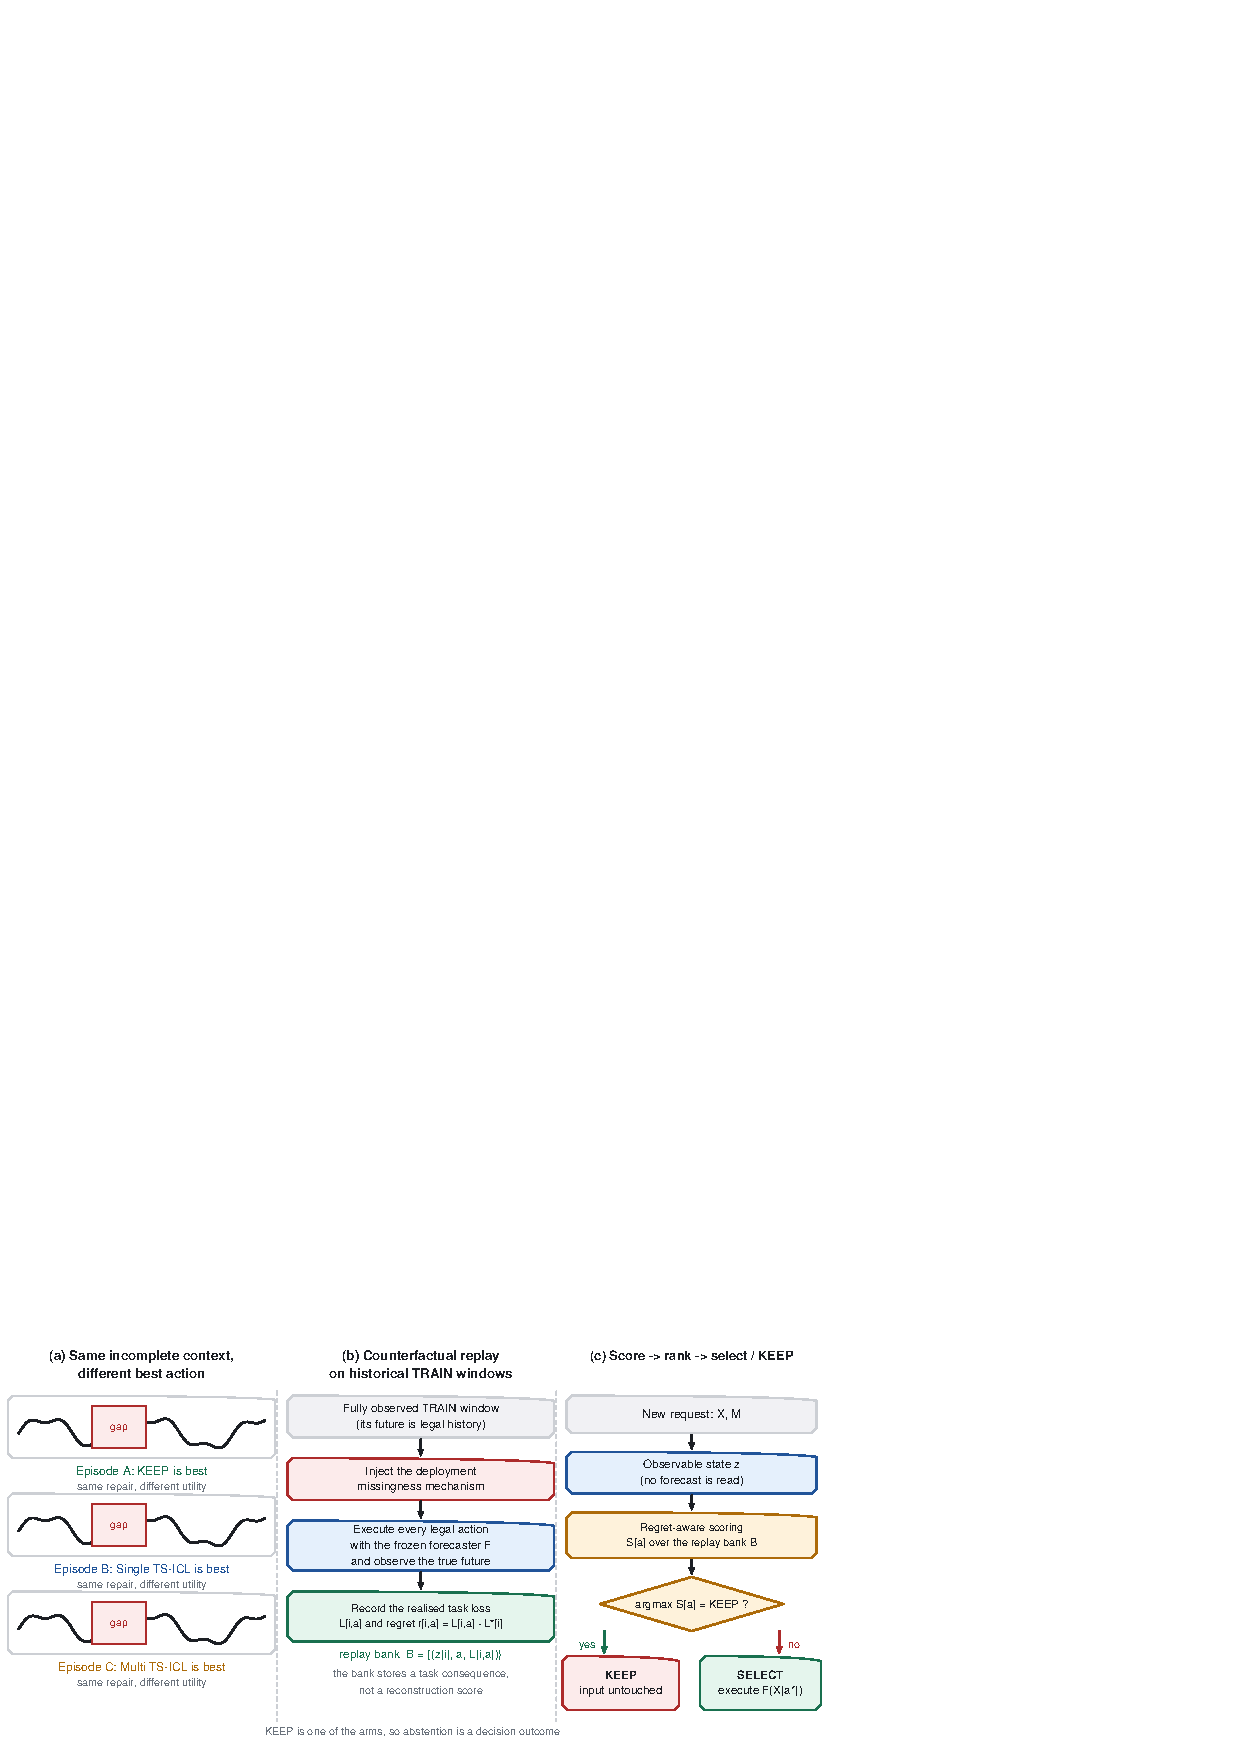
\includegraphics[width=0.87\textwidth]{figure/fig1_selective_governance.pdf}
  \caption{Repair is treated as a selective forecasting decision rather than a mandatory
  preprocessing operation. \textbf{(a)}~Three episodes share the same incomplete-context
  problem but have different best actions, so the utility of a repair is episode
  dependent. \textbf{(b)}~Historical TRAIN windows are replayed as pseudo-deployments:
  the deployment missingness mechanism is injected and every legal action is really
  executed with the frozen forecaster, yielding the realised utility $g_{i,a}$.
  \textbf{(c)}~A new request is matched against the replay bank, and an action is taken
  only if its conservative utility is positive; otherwise the system abstains and returns
  the reference forecast.}
  \label{fig:concept}
\end{figure}

% ===========================================================================
\section{Related Work}
\label{sec:related}

\subsection{Time-Series Imputation}
Reconstruction-oriented imputation is a mature line. BRITS~\citep{cao2018brits}
performs bidirectional recurrent imputation and was an early demonstration that temporal
consistency improves reconstruction. CSDI~\citep{tashiro2021csdi} replaces the
deterministic mapping with a conditional score-based diffusion model, producing
probabilistic imputations, and generative or self-attention variants such as
GAIN~\citep{yoon2018gain} and SAITS~\citep{du2023saits} explore related alternatives.
Most recently, T1~\citep{park2026t1} targets diverse missing patterns and heavy missing
ratios by binding CNN channels to attention heads, so that cross-variable information
transfer can be selectively suppressed when a channel's temporal evidence is corrupted.
All of these methods are evaluated primarily on reconstruction error. We use BRITS, CSDI,
and T1 as published baselines and, in \S\ref{sec:exp-recutility}, measure directly whether
their reconstruction advantage translates into forecasting utility for a frozen \tsfm{}.

\subsection{Task-Oriented Imputation}
Task-oriented imputation evaluation~\citep{wang2024taskoriented} reframes the objective:
rather than asking how well missing values are recovered, it estimates how much a given
imputation strategy helps a downstream task, and reports that strategy rankings under
reconstruction and under task utility can disagree. This is the closest prior work to our
motivation. Our problem differs in kind rather than in degree: task-oriented evaluation
still produces a \emph{strategy-level} score and a fused imputation, whereas we ask
whether a specific legal action should be executed for a specific episode, and we
explicitly allow the answer to be ``no action''. We also restrict the final forecast to
one really executed input version, so no output fusion or post-hoc correction can
contribute to the reported numbers.

\subsection{Data-Centric Adaptation of Time-Series Foundation Models}
TATO~\citep{qiu2026tato} searches over transformation pipelines so that heterogeneous
domains can be served by a single frozen \tsfm{}, selecting pipelines by historical task
performance. This established data-to-model adaptation as an effective paradigm, so
``adapting the data instead of the model'' is no longer a contribution by itself.
In-context adaptation~\citep{tsicl2026} provides a related route in which the context
itself carries the task specification. Relative to both, our object of study is the
\emph{decision} layer: given a catalog of already-available legal interventions, which
one, if any, should be applied to \emph{this} incomplete context. Work on sequential
evidence acquisition and decision value~\citep{he2024dime,kang2020forecastwithforecasts}
formalises when information is worth its cost; we deliberately keep our selection rule a
simple conservative heuristic rather than claiming an information-theoretic optimum, and
report its full cost accounting in \S\ref{sec:exp-efficiency}.

% ===========================================================================
\section{Problem Formulation and Method}
\label{sec:method}

\begin{figure}[t]
  \centering
  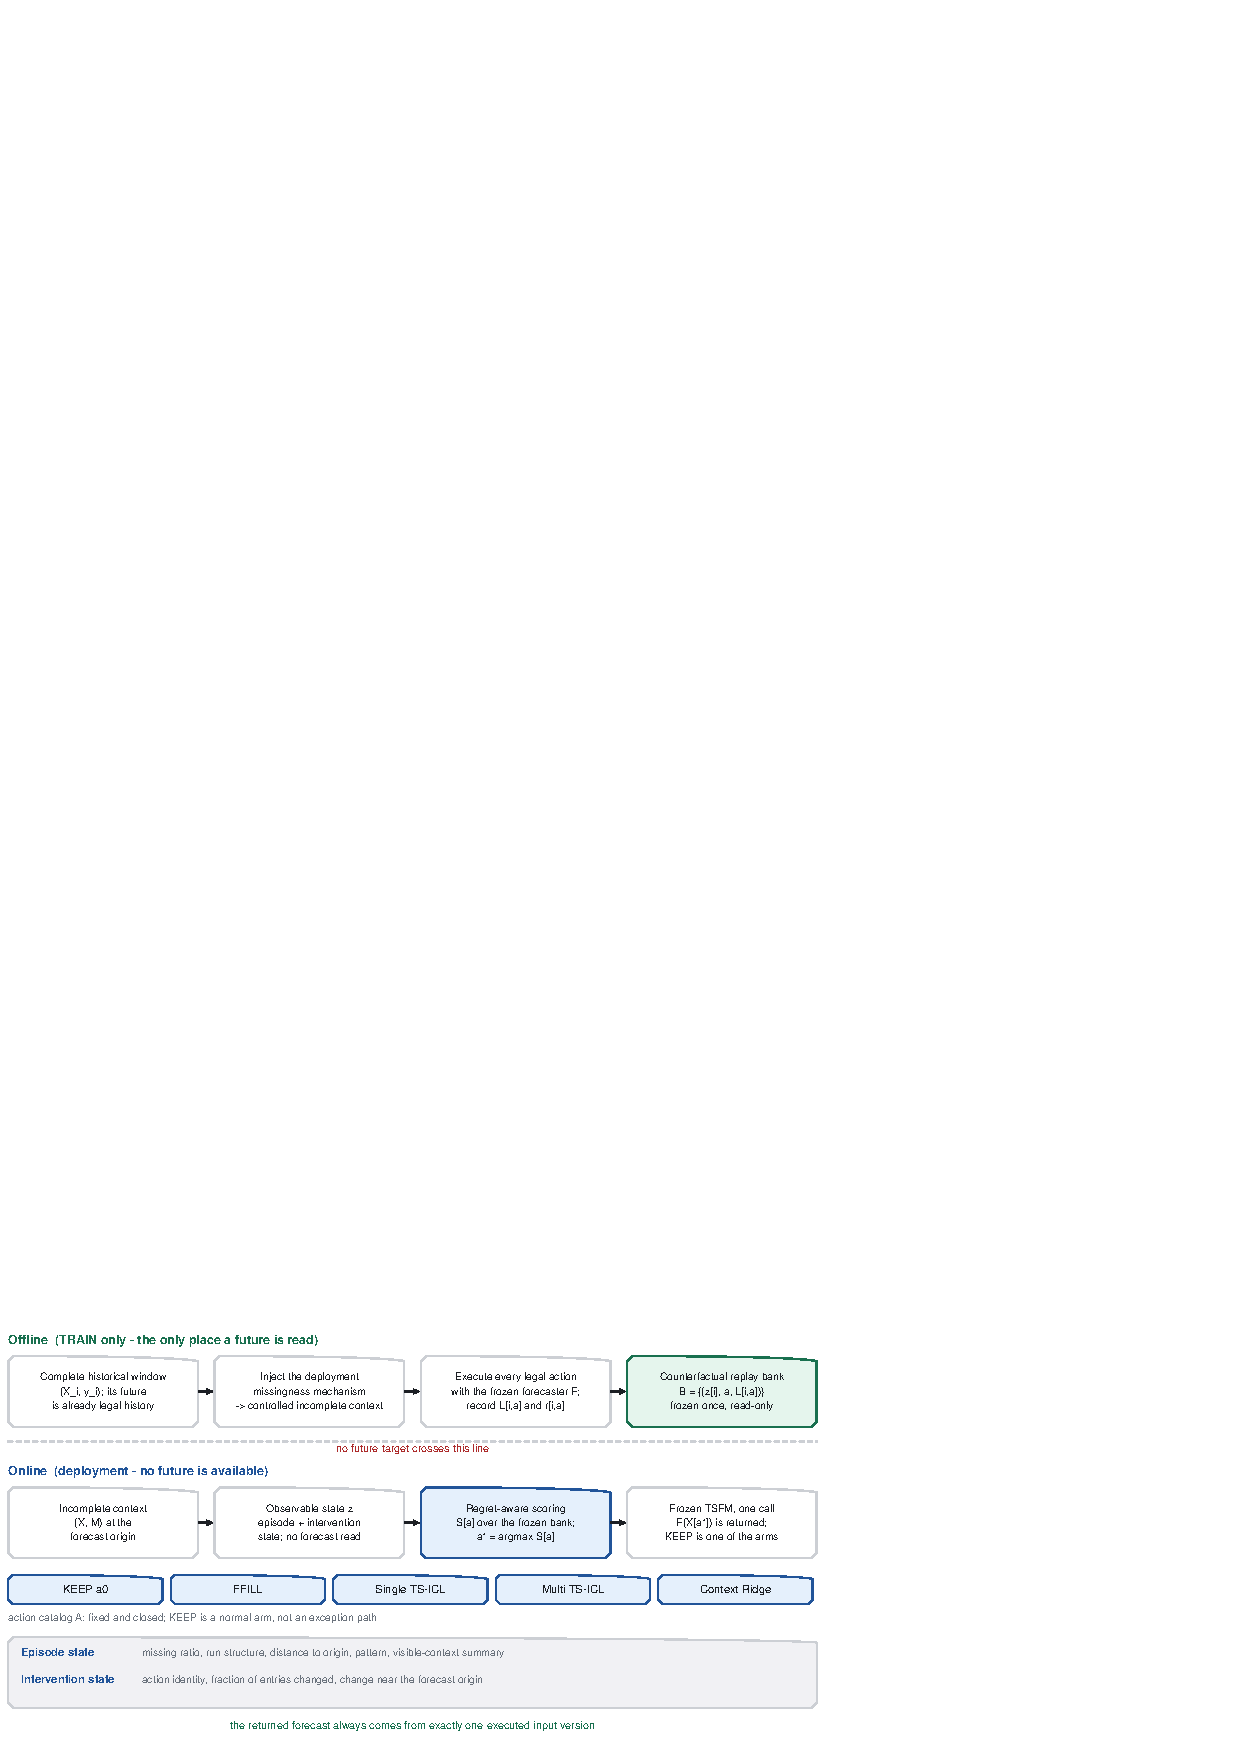
\includegraphics[width=0.79\textwidth]{figure/fig2_introact_architecture.pdf}
  \caption{Architecture of \introact{}. A deployment request produces a reference
  forecast and a set of materialised legal input versions. In parallel, a counterfactual
  replay bank is built once from TRAIN windows. The observable task state of the request
  is matched against the bank, each candidate action receives a conservative utility
  score, and exactly one action is executed --- or the system abstains. The returned
  forecast always comes from a single really executed input version.}
  \label{fig:arch}
\end{figure}

\subsection{Problem Formulation}
\label{sec:method-problem}
Let $X \in \mathbb{R}^{C \times L}$ be the multivariate context available at the forecast
origin, with observation mask $M \in \{0,1\}^{C \times L}$, and let
$Y \in \mathbb{R}^{C \times H}$ be the future target, which is \emph{never} available to
the decision procedure. Let $F$ be a frozen time-series foundation model with fixed
parameters; $F$ maps a complete-enough input to a forecast
$p = F(X) \in \mathbb{R}^{C \times H}$. Let
$\calA = \{a_0, a_1, \dots, a_K\}$ be a fixed catalog of legal governance actions, where
each $a$ materialises a legal input version $X^{a}$ from $(X, M)$, and $a_0$ is the
\emph{reference} action (the untouched input, i.e.\ KEEP). Let $\loss(p, Y)$ be a
forecasting loss. The task is to choose
\begin{equation}
  a^\star(X, M) \;\in\; \calA \cup \{\textsc{Abstain}\},
  \qquad
  a^\star \text{ must not depend on } Y ,
  \label{eq:objective}
\end{equation}
so as to improve $\loss(F(X^{a^\star}), Y)$ relative to the reference
$\loss(F(X^{a_0}), Y)$, while keeping the number of frozen-model calls small and avoiding
harmful interventions.

Three structural constraints distinguish this from ordinary imputation. First, \emph{no
valid observation may be overwritten}: every $X^{a}$ differs from $X^{a_0}$ only at
positions where $M = 0$. Second, \emph{the future is unavailable}: no candidate forecast
may be inspected before an action is chosen, and features may not be computed from
forecasts of non-selected candidates. Third, \emph{abstention is legal}: leaving the
input untouched is a valid outcome, and the system is not required to act.

\subsection{Counterfactual Replay}
\label{sec:method-replay}
The central difficulty is that the quantity we care about,
$g_a = \loss(F(X^{a_0}), Y) - \loss(F(X^{a}), Y)$, depends on $Y$ and therefore cannot be
observed at deployment. Our remedy is to obtain it from the past. For a historical
window whose forecast target is already part of the legally visible history, the same
quantity is computable: the window is fully observed, its future is known, and it can
therefore be re-enacted as a \emph{pseudo-deployment}.

Concretely, for a historical window $i$ we take its complete context $X_i$ and its
already-realised future $y_i$, inject the \emph{same} missingness mechanism that
deployment uses (the mechanism is fixed before any method is run, see
\S\ref{sec:exp-setup}), obtaining an incomplete input $(X_i, M_i)$, and then really
execute every action $a \in \calA$ with the frozen forecaster $F$:
\begin{equation}
  g_{i,a} \;=\; \loss\!\left(F(X_i^{a_0}),\, y_i\right) \;-\; \loss\!\left(F(X_i^{a}),\, y_i\right) .
  \label{eq:replay-gain}
\end{equation}
Each executed pseudo-deployment contributes a triple
\begin{equation}
  \calB \;=\; \bigl\{\, (z_i,\, a,\, g_{i,a}) \,\bigr\},
  \label{eq:replay-bank}
\end{equation}
where $z_i$ is the \emph{observable} task state of the pseudo-deployment (\S\ref{sec:method-state}).
The resulting bank is a record of what actually happened when each legal intervention was
applied to a real historical window under the deployment missingness mechanism. It is not
a model of the data, and $g_{i,a}$ is not a reconstruction score: it is the realised
change in forecasting loss.

Because $y_i$ belongs to TRAIN history, no test-time label is ever consulted. The bank is
built once, offline, and is then frozen; deployment reads it but never writes to it.
Figure~\ref{fig:concept}(b) summarises this construction.

\subsection{Task-State Matching}
\label{sec:method-state}
A request is answered by retrieving historical replays that resemble it, so the state
representation has to describe both \emph{how incomplete} the request is and \emph{what
the candidate intervention would change}. We deliberately avoid a learned encoder and use
four groups of lightweight, directly computable features:

\begin{itemize}\itemsep1pt
  \item \textbf{A --- Mask state}: overall missing ratio, longest missing run, number of
  missing runs, distance from the nearest missing position to the forecast origin, a
  target-only/shared indicator, and a tail-missing indicator.
  \item \textbf{B --- Visible-context state}, computed only from values that are actually
  visible: robust scale, linear trend, lag-1 autocorrelation, seasonal autocorrelation,
  recent level shift, and recent volatility.
  \item \textbf{C --- Intervention state}: for each candidate version $X^{a}$ relative to
  the reference $X^{a_0}$, the mean absolute change, maximum absolute change, fraction of
  changed positions, change trend, and the change within the last-observed region. These
  describe the difference between two \emph{inputs}, never a difference between forecasts.
  \item \textbf{D --- Reference-forecast state}: obtained from the single legal reference
  forecast $p_0 = F(X^{a_0})$ only --- its mean, range, slope, first-step jump from the
  last visible observation, and roughness.
\end{itemize}

Group~D deserves emphasis. We execute only the reference forecast before deciding; we do
not run the non-selected candidates' forecasts to build features. This keeps the state
observable under the deployment contract of \S\ref{sec:method-problem} and keeps the
number of frozen-model calls at the level reported in \S\ref{sec:exp-efficiency}. All
continuous features are standardised using statistics fitted on the replay-fit portion of
TRAIN only; similarity is standardised Euclidean distance, with no learned metric.
Retrieval is performed \emph{per action}, so for action $a$ the neighbourhood $\calN_a$
contains only historical replays of the same action, and
\begin{equation}
  w_i \;=\; \exp\!\left(-\,d_i / \tau\right), \qquad
  \tau \;=\; \operatorname{median}_{i \in \calN_a} d_i + \epsilon .
  \label{eq:weights}
\end{equation}
The bandwidth $\tau$ is not tuned: it is set from the query's own neighbourhood, so that
the only searched hyperparameter is $K \in \{8, 16, 32\}$.

\subsection{Conservative Intervention}
\label{sec:method-gate}
For a new request and candidate action $a$, the matched replays give a local estimate of
the utility of $a$,
\begin{equation}
  \hat\mu_a \;=\; \frac{\sum_{i \in \calN_a} w_i\, g_{i,a}}{\sum_{i \in \calN_a} w_i},
  \qquad
  \hat\sigma_a^2 \;=\; \frac{\sum_{i \in \calN_a} w_i\,(g_{i,a} - \hat\mu_a)^2}{\sum_{i \in \calN_a} w_i},
  \qquad
  n_{\mathrm{eff},a} \;=\; \frac{\bigl(\sum_i w_i\bigr)^2}{\sum_i w_i^2} .
  \label{eq:local-mean}
\end{equation}
A positive mean alone is not a sufficient reason to act: local historical evidence can be
thin or contradictory, and acting on a noisy positive estimate is exactly how a repair
becomes harmful. We therefore score each action by a lower-confidence quantity
\begin{equation}
  S_a \;=\; \hat\mu_a \;-\; \beta\,\frac{\hat\sigma_a}{\sqrt{n_{\mathrm{eff},a}}},
  \label{eq:conservative-score}
\end{equation}
and take
\begin{equation}
  a^\star \;=\;
  \begin{cases}
    \arg\max_{a \in \calA} S_a, & \max_{a \in \calA} S_a > 0,\\[2pt]
    a_0 \ (\textsc{Abstain}),   & \text{otherwise}.
  \end{cases}
  \label{eq:act-abstain}
\end{equation}
The reference action $a_0$ is always legal, so abstention never fails: when the evidence
is insufficient or points to harm, the system returns the untouched input. The
conservatism level $\beta \in \{0, 1, 1.64\}$ and the neighbourhood size $K$ are the only
tuned quantities; both are selected on a held-out TRAIN gate (\S\ref{sec:exp-setup}) and
then frozen. $S_a$ is a heuristic score, not a calibrated lower bound on $g_a$; we report
its sign agreement with realised utility in \S\ref{sec:exp-governance} and do not claim
coverage guarantees.

\subsection{Deployment and Complexity}
\label{sec:method-deploy}
A deployment request is served in eight steps: read the visible context and mask; execute
the reference action and obtain $p_0$; materialise the legal candidate input versions;
extract the observable state $z$; query the frozen replay bank; compute $S_a$ for every
candidate; abstain if $\max_a S_a \le 0$, otherwise execute $a^\star$; and return
$F(X^{a^\star})$. The frozen backbone is called once for the reference and once for the
selected action, so a request costs one or two \tsfm{} forecasts; the exact distribution
is reported in \S\ref{sec:exp-efficiency}. There is no ensemble, no output correction, no
residual model, and no parameter update. Cost accounting is deliberately explicit:
candidate materialisation, imputer runtime, the reference \tsfm{} call, the selected
\tsfm{} call, selector overhead, and total request wall-clock are recorded separately, and
no component is booked as free because a cached artefact happened to exist.

% ===========================================================================
\section{Experiments}
\label{sec:exp}

\subsection{Experimental Setup}
\label{sec:exp-setup}
\paragraph{Datasets and backbones.}
The main matrix uses \ph{N-DATASETS} public forecasting sources: ETTh1, ETTh2, ETTm1,
ETTm2, Electricity~\citep{uci_electricity}, Exchange~\citep{lai2018lstnet},
Traffic~\citep{pems}, and Weather~\citep{wu2021autoformer}. Three frozen \tsfm{} families
are used: Chronos-Bolt~\citep{chronosbolt2025} (\emph{Bolt}),
TimesFM-2.5~\citep{das2024timesfm} (\emph{TimesFM}), and Chronos-2~\citep{chronos2_2025}
(\emph{Chronos-2}). Bolt and TimesFM are used for method development; Chronos-2 takes no
part in method design, and only after the \introact{} configuration is completely frozen
do we use the identical algorithm and hyperparameters to build its legal TRAIN replay bank
and enter the main experiment. This tests method transfer across frozen \tsfm{} families
rather than per-backbone tuning. Context length is $L = 512$, main horizons are
$H \in \{96, 192\}$, and longer horizons appear only in Appendix~\ref{app:horizons}.

\paragraph{Governance actions.}
The catalog is fixed at five legal actions,
$\calA = \{\textsc{Keep},\ \textsc{Ffill},\ \textsc{Single TS-ICL},\ \textsc{Multi TS-ICL},\ \textsc{Context Ridge}\}$,
with \textsc{Keep} as the reference $a_0$. It is deliberately not enlarged: the
contribution under test is governance, not imputer architecture. A complete and
valid input is always mapped to \textsc{Keep}; unsupported, aliased, and failed actions
are recorded rather than silently dropped.

\paragraph{Missingness protocol.}
Four deterministic patterns are frozen before any method runs: \textbf{P1 point missing};
\textbf{P2 target block} (a contiguous block missing on the target variable);
\textbf{P3 shared block} (several visible variables missing over the same interval); and
\textbf{P4 tail missing} (a block adjacent to the forecast origin, modelling observations
that have not arrived). Every mask is derived by a deterministic hash of
\texttt{source + parent + origin + horizon + pattern + protocol\_seed} and is never moved
after forecasts are seen. The main experiment uses $10\%$ severity, matching the scale of
the preceding controlled-deletion work; \S\ref{sec:exp-robust} adds $30\%$ and $50\%$.

\paragraph{Splits.}
Only legal TRAIN parents are used. Within TRAIN, parents are sorted by source and time and
divided into \emph{replay-fit} ($\sim$60\%, used to build the replay bank, train
baselines, and fit feature normalisation), \emph{gate} ($\sim$20\%, used to select $K$,
$\beta$, and any legal baseline hyperparameter), and \emph{TRAIN-eval} ($\sim$20\%, the
final internal acceptance check before freezing). Purging is enforced at $L + H$ and no
parent's masks, patterns, or horizons cross a split boundary. TRAIN-eval targets may be
used for evaluation but never to refit the selector. Replay pseudo-deployment severities
are drawn from $\{10\%, 30\%, 50\%\}$ by deterministic hash, so the full method is a single
configuration that is never retuned per severity.

\paragraph{Baselines and controls.}
Five published baselines are fixed in advance and never swapped after results are seen:
BRITS~\citep{cao2018brits}, CSDI~\citep{tashiro2021csdi}, TOI/generalized
representers~\citep{wang2024taskoriented}, T1~\citep{park2026t1}, and
TATO~\citep{qiu2026tato}. All five appear in every main-text experiment. Alongside them we
report three controls that are not claimed as published baselines: \textsc{Native Keep}
(no governance), \textsc{Best Fixed} (one action chosen on TRAIN and applied to every
request, testing whether instance-level selection is necessary at all), and
\textbf{R2-CART}, the strongest simple selector inherited from the preceding development
cycle, which \introact{} must beat if a more elaborate procedure is to be justified.
Finally, a \emph{Catalog Oracle} chooses the best of the five legal actions using the
future target; it is a diagnostic upper reference only, never deployable, never part of
any average rank, and rendered in grey italics. Trainable imputers (BRITS, CSDI, T1) are
trained on TRAIN only with a TRAIN mixture over the same three severities. Because our
$L = 512$ task differs from the TATO paper's setting, we report TATO explicitly as
\emph{under our $L{=}512$ protocol} and never as a full replication.

\paragraph{Metrics, aggregation, and statistics.}
The primary metric is MASE~\citep{hyndman2006mase}, averaged source-macro: first over
parents, then over sources, with the eight sources equally weighted. Secondary metrics are
MSE, MAE, and RMSSE. MAPE is not a headline metric because it is unstable near zero, CRPS
is not used because not every backbone or baseline exposes comparable probabilistic
forecasts, and QLIKE is deferred to the finance case study (Appendix~\ref{app:finance}).
Efficiency is reported separately and never folded into an accuracy score. The primary
statistical unit is the parent: we use paired cluster bootstrap with \ph{N-BOOTSTRAP}
resamples over parent blocks for 95\% confidence intervals on source-macro MASE
differences against each baseline, with Holm correction~\citep{holm1979simple} across
baselines, and additionally report average rank and the number of won cells over
source $\times$ backbone $\times$ horizon $\times$ pattern. Mask variants of the same
parent are never treated as independent samples.

\subsection{Main Results}
\label{sec:exp-main}
\emph{Does \introact{} improve incomplete-input forecasting across datasets and frozen
\tsfm{} backbones compared with recent task-oriented, imputation, and TSFM-adaptation
methods?}

Table~\ref{tab:main} reports the main comparison under the 10\% severity condition, with
all eight sources, three backbones, two horizons, and four patterns. \ph{MAIN-READING}.
\ph{MAIN-BACKBONE-CONSISTENCY}. \ph{MAIN-T1TATO}. \ph{MAIN-R2CART}. \ph{MAIN-RANK}.
Per-dataset MAE and RMSSE tables are deferred to Appendix~\ref{app:datasets}.

\begin{table}[t]
  \caption{Main results at 10\% missingness; MASE is source-macro averaged and lower is
  better. \best{Bold} is the best deployable method, \second{underline} the second best.
  The oracle row uses future targets for diagnosis only, is not deployable, and is excluded
  from ranks and from all claims.}
  \label{tab:main}
  \centering
  \small
  \setlength{\tabcolsep}{4pt}
\resizebox{\textwidth}{!}{\begin{tabular}{lcccccc}
    \toprule
    Method & Bolt MASE $\downarrow$ & TimesFM MASE $\downarrow$ & Chronos-2 MASE $\downarrow$
           & Overall MASE $\downarrow$ & MSE $\downarrow$ & Avg.\ Rank $\downarrow$ \\
    \midrule
    Native KEEP      & \ph{KEEP-BOLT}  & \ph{KEEP-TF}  & \ph{KEEP-CH2}  & \ph{KEEP-OVR}  & \ph{KEEP-MSE}  & \ph{KEEP-RANK} \\
    Best Fixed       & \ph{BF-BOLT}    & \ph{BF-TF}    & \ph{BF-CH2}    & \ph{BF-OVR}    & \ph{BF-MSE}    & \ph{BF-RANK} \\
    R2-CART          & \ph{R2-BOLT}    & \ph{R2-TF}    & \ph{R2-CH2}    & \ph{R2-OVR}    & \ph{R2-MSE}    & \ph{R2-RANK} \\
    BRITS            & \ph{BRITS-BOLT} & \ph{BRITS-TF} & \ph{BRITS-CH2} & \ph{BRITS-OVR} & \ph{BRITS-MSE} & \ph{BRITS-RANK} \\
    CSDI             & \ph{CSDI-BOLT}  & \ph{CSDI-TF}  & \ph{CSDI-CH2}  & \ph{CSDI-OVR}  & \ph{CSDI-MSE}  & \ph{CSDI-RANK} \\
    TOI              & \ph{TOI-BOLT}   & \ph{TOI-TF}   & \ph{TOI-CH2}   & \ph{TOI-OVR}   & \ph{TOI-MSE}   & \ph{TOI-RANK} \\
    T1               & \ph{T1-BOLT}    & \ph{T1-TF}    & \ph{T1-CH2}    & \ph{T1-OVR}    & \ph{T1-MSE}    & \ph{T1-RANK} \\
    TATO             & \ph{TATO-BOLT}  & \ph{TATO-TF}  & \ph{TATO-CH2}  & \ph{TATO-OVR}  & \ph{TATO-MSE}  & \ph{TATO-RANK} \\
    \midrule
    \rowcolor{bestgray}\introact{}      & \ph{OURS-BOLT}  & \ph{OURS-TF}  & \ph{OURS-CH2}  & \ph{OURS-OVR}  & \ph{OURS-MSE}  & \ph{OURS-RANK} \\
    \midrule
    Catalog Oracle   & \oracle{\ph{ORACLE-BOLT}} & \oracle{\ph{ORACLE-TF}}
      & \oracle{\ph{ORACLE-CH2}} & \oracle{\ph{ORACLE-OVR}} & \oracle{\ph{ORACLE-MSE}} & \oracle{--} \\
    \bottomrule
  \end{tabular}}
\end{table}

\subsubsection{Efficiency and Deployment Cost}
\label{sec:exp-efficiency}
Table~\ref{tab:efficiency} separates offline cost from online cost. Offline
training/search is the one-off cost of fitting trainable imputers or running a
transformation search; online cost covers candidate construction, frozen-model calls, and
end-to-end request latency. Cached historical artefacts are never booked as zero, and
batch-averaged latency is never presented as a per-request guarantee; cold start is
reported separately and never merged into hot latency.

\begin{table}[t]
  \caption{Deployment cost, offline and online kept separate. Latency percentiles are
  per request and exclude cold start, reported on its own line. Lower is better except for
  the call count.}
  \label{tab:efficiency}
  \centering
  \small
  \setlength{\tabcolsep}{4pt}
\resizebox{\textwidth}{!}{\begin{tabular}{lcccccc}
    \toprule
    Method & Offline train/search & Candidate constr. & TSFM calls/req.\ & Mean lat.\ $\downarrow$ & P95 $\downarrow$ & Max $\downarrow$ \\
    \midrule
    BRITS       & \ph{BRITS-OFF} & \ph{BRITS-CAND} & \ph{BRITS-CALLS} & \ph{BRITS-MEAN} & \ph{BRITS-P95} & \ph{BRITS-MAX} \\
    CSDI        & \ph{CSDI-OFF}  & \ph{CSDI-CAND}  & \ph{CSDI-CALLS}  & \ph{CSDI-MEAN}  & \ph{CSDI-P95}  & \ph{CSDI-MAX} \\
    TOI         & \ph{TOI-OFF}   & \ph{TOI-CAND}   & \ph{TOI-CALLS}   & \ph{TOI-MEAN}   & \ph{TOI-P95}   & \ph{TOI-MAX} \\
    T1          & \ph{T1-OFF}    & \ph{T1-CAND}    & \ph{T1-CALLS}    & \ph{T1-MEAN}    & \ph{T1-P95}    & \ph{T1-MAX} \\
    TATO        & \ph{TATO-OFF}  & \ph{TATO-CAND}  & \ph{TATO-CALLS}  & \ph{TATO-MEAN}  & \ph{TATO-P95}  & \ph{TATO-MAX} \\
    \rowcolor{bestgray}\introact{} & \ph{OURS-OFF}  & \ph{OURS-CAND}  & \ph{OURS-CALLS}  & \ph{OURS-MEAN}  & \ph{OURS-P95}  & \ph{OURS-MAX} \\
    \midrule
    \multicolumn{7}{l}{\footnotesize Cold start: \ph{COLDSTART} \quad
    Failure/timeout share: \ph{FAILRATE}} \\
    \bottomrule
  \end{tabular}}
\end{table}

\subsection{Reconstruction Is Not Forecast Utility}
\label{sec:exp-recutility}
\emph{Does better reconstruction imply better forecasting for a frozen \tsfm{}?}

This experiment reuses the predictions produced by the main experiment; no protocol is
changed. Because the artificially hidden positions are known, the reconstruction error
$E^{\mathrm{rec}}$ is computable, and the forecasting effect is
$\Delta L^{\mathrm{forecast}} = L_{\textsc{Keep}} - L_{\text{method}}$. All five published
baselines enter. Figure~\ref{fig:recutil} plots reconstruction improvement against
forecasting improvement, one point per parent--method pair, with identical axis
definitions across backbones; the paired numbers and the discordant rate are in
Table~\ref{tab:recutil}.

\begin{table}[t]
  \caption{Reconstruction quality versus forecasting utility, summarised here; the full
  paired table is Table~\ref{tab:app-recutils} in Appendix~\ref{app:recutils}.}
  \label{tab:recutil}
  \centering
  \small
  \setlength{\tabcolsep}{4pt}
\resizebox{\textwidth}{!}{\begin{tabular}{lcccc}
    \toprule
    Backbone & Rec.\ MSE $\downarrow$ & Rec.\ MAE $\downarrow$ & Forecast Gain $\uparrow$ & Discordant Rate $\downarrow$ \\
    \midrule
    Bolt        & \ph{BOLT-REC-MSE}  & \ph{BOLT-REC-MAE}  & \ph{BOLT-GAIN}  & \ph{BOLT-DISCORDANT} \\
    TimesFM     & \ph{TF-REC-MSE}    & \ph{TF-REC-MAE}    & \ph{TF-GAIN}    & \ph{TF-DISCORDANT} \\
    Chronos-2   & \ph{CH2-REC-MSE}   & \ph{CH2-REC-MAE}   & \ph{CH2-GAIN}   & \ph{CH2-DISCORDANT} \\
    \bottomrule
  \end{tabular}}
\end{table}

\begin{figure}[t]
  \centering
  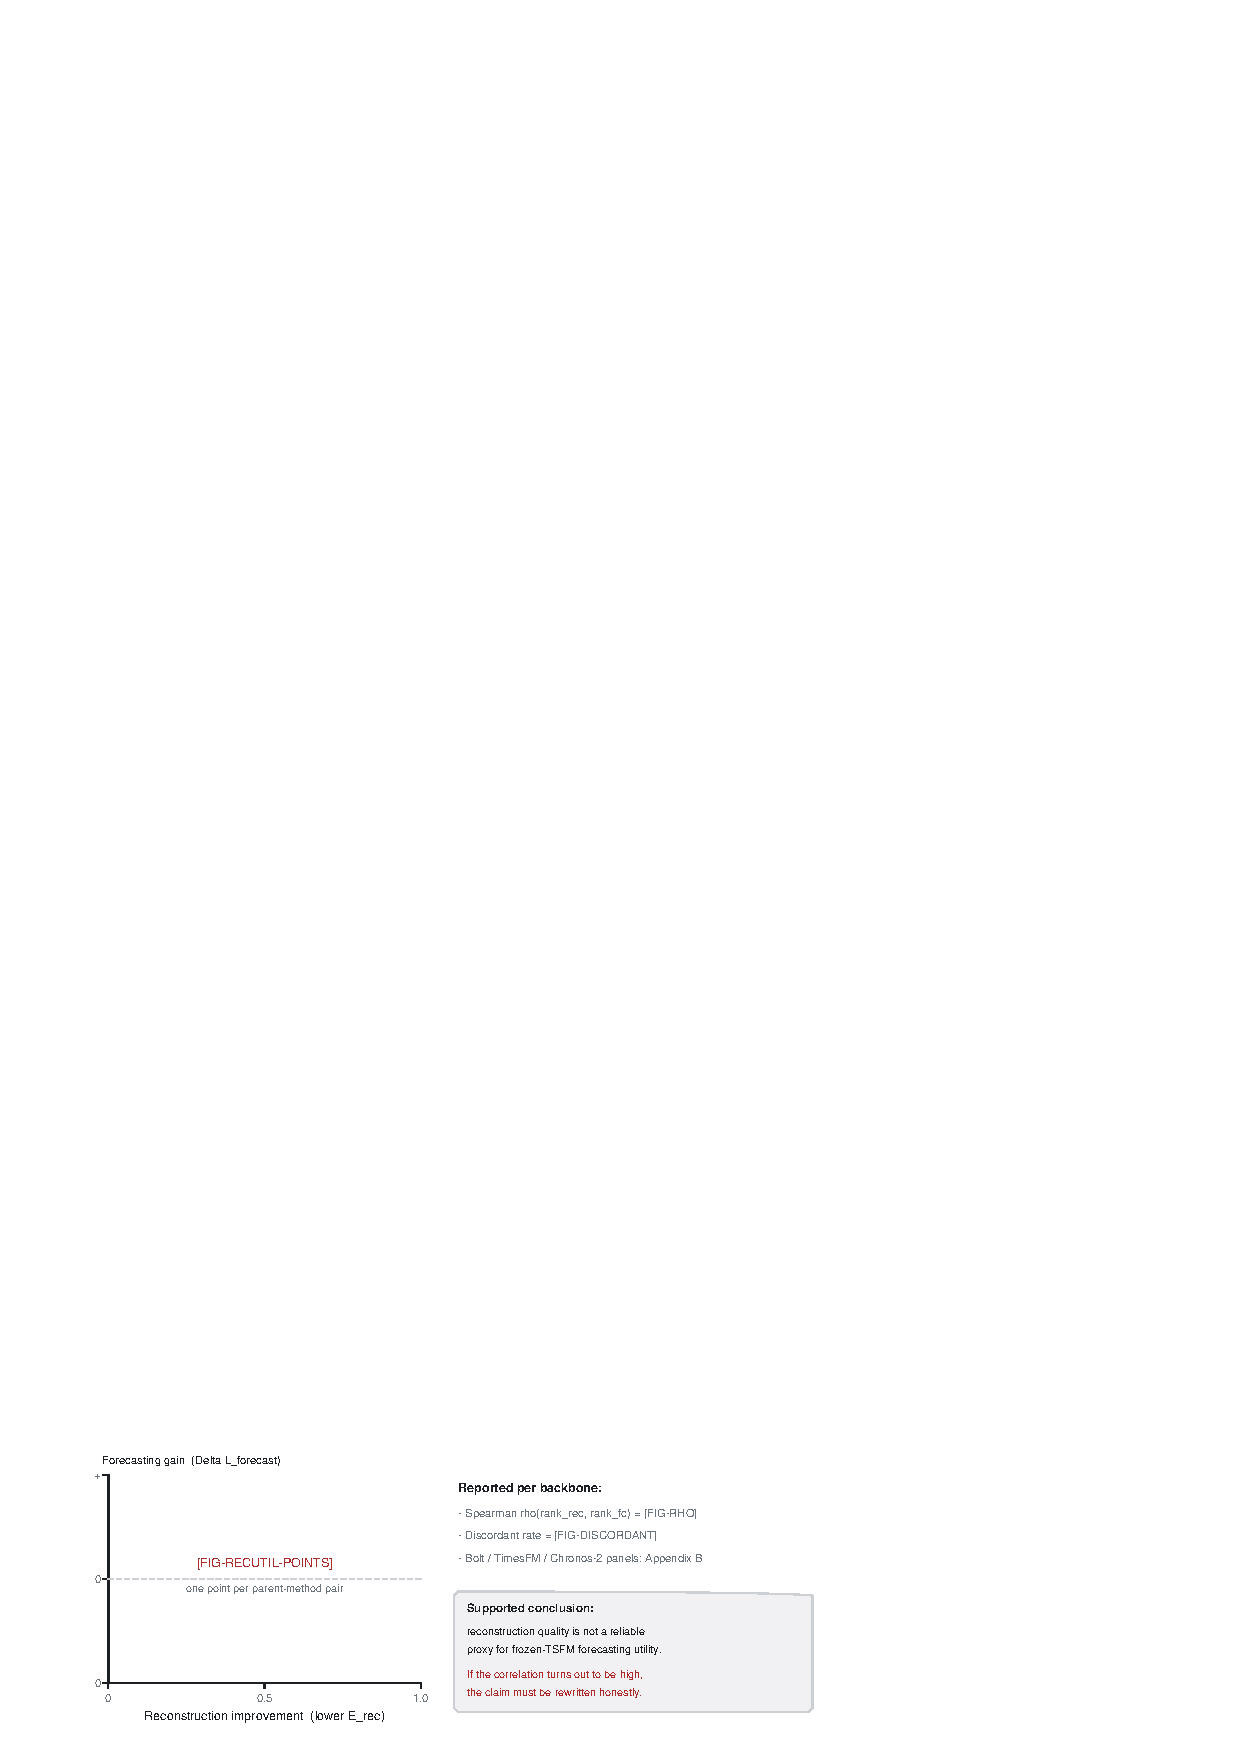
\includegraphics[width=0.66\textwidth]{figure/fig3_reconstruction_vs_utility.pdf}
  \caption{Reconstruction improvement against forecasting improvement, one point per
  parent--method pair, identical axes for every backbone. The panel is a placeholder until
  the main experiment produces the underlying CSV.}
  \label{fig:recutil}
\end{figure}

The claim this experiment can support is deliberately narrow: \emph{reconstruction quality
is not a reliable proxy for frozen-\tsfm{} forecasting utility}. If the measured correlation
turns out to be high, this conclusion must be rewritten rather than softened.

\subsection{When Should We Intervene?}
\label{sec:exp-governance}
\emph{Can historical counterfactual utility support instance-level intervention
decisions, and does abstention reduce harmful governance?}

All five published baselines enter. We report four governance diagnostics: the
\emph{intervention rate} (fraction of requests whose input was actually changed); the
\emph{harmful intervention rate}
$\mathrm{HIR} = |\{i : L_{m,i} > L_{\textsc{Keep},i}\}| / N$, reported both
unconditionally and restricted to windows where an intervention occurred; the
\emph{harmful loss}
$\mathrm{HL} = \frac{1}{N}\sum_i \max(0, L_{m,i} - L_{\textsc{Keep},i})$; and the
\emph{catalog gap closed}
\begin{equation}
  \mathrm{CGC} \;=\; \frac{L_{\textsc{Keep}} - L_m}{L_{\textsc{Keep}} - L_{\mathrm{oracle}}},
  \qquad
  L_{\mathrm{oracle}} = \min_{a \in \calA} L_a ,
  \label{eq:cgc}
\end{equation}
computed only on improvable windows where the oracle strictly beats \textsc{Keep}. We call
it the \emph{catalog} gap because T1, CSDI and the other baselines can produce inputs
outside the five-arm catalog; it is not a universal oracle gap and we do not describe it
as one. Figure~\ref{fig:governance} in Appendix~\ref{app:governance-fig} shows the
per-method harmful loss and the realised utility against the binned conservative score.

\begin{table}[t]
  \caption{Selective governance diagnostics. HIR and harmful loss measure harm relative
  to \textsc{Native Keep}; catalog gap closed measures the share of the achievable five-arm
  improvement that was captured.}
  \label{tab:governance}
  \centering
  \small
  \setlength{\tabcolsep}{4pt}
\resizebox{\textwidth}{!}{\begin{tabular}{lccccc}
    \toprule
    Method & MASE $\downarrow$ & Intervention Rate & HIR $\downarrow$ & Harmful Loss $\downarrow$ & Catalog Gap Closed $\uparrow$ \\
    \midrule
    Best Fixed       & \ph{BF-MASE}    & \ph{BF-IR}    & \ph{BF-HIR}    & \ph{BF-HL}    & \ph{BF-CGC} \\
    R2-CART          & \ph{R2-MASE}    & \ph{R2-IR}    & \ph{R2-HIR}    & \ph{R2-HL}    & \ph{R2-CGC} \\
    BRITS            & \ph{BRITS-MASE} & \ph{BRITS-IR} & \ph{BRITS-HIR} & \ph{BRITS-HL} & \ph{BRITS-CGC} \\
    CSDI             & \ph{CSDI-MASE}  & \ph{CSDI-IR}  & \ph{CSDI-HIR}  & \ph{CSDI-HL}  & \ph{CSDI-CGC} \\
    TOI              & \ph{TOI-MASE}   & \ph{TOI-IR}   & \ph{TOI-HIR}   & \ph{TOI-HL}   & \ph{TOI-CGC} \\
    T1               & \ph{T1-MASE}    & \ph{T1-IR}    & \ph{T1-HIR}    & \ph{T1-HL}    & \ph{T1-CGC} \\
    TATO             & \ph{TATO-MASE}  & \ph{TATO-IR}  & \ph{TATO-HIR}  & \ph{TATO-HL}  & \ph{TATO-CGC} \\
    \midrule
    \rowcolor{bestgray}\introact{}      & \ph{OURS-MASE}  & \ph{OURS-IR}  & \ph{OURS-HIR}  & \ph{OURS-HL}  & \ph{OURS-CGC} \\
    \bottomrule
  \end{tabular}}
\end{table}

\subsection{Robustness to Missingness}
\label{sec:exp-robust}
\emph{Does the same frozen governance policy remain useful as missingness becomes more
severe and structurally different?}

All five published baselines enter. Severities are $10\%$, $30\%$ and $50\%$, crossed with
the four patterns and the three backbones. No method is retuned: \introact{} reuses the
$K$ and $\beta$ frozen after the TRAIN gate, and the baselines reuse the models and rules
fixed on TRAIN. Complete numbers are in Appendix~\ref{app:severity}, and
Figure~\ref{fig:robust} in Appendix~\ref{app:robust-fig} shows the severity trend.

\begin{table}[t]
  \caption{Robustness to missingness severity. The worst-case column is the largest
  degradation relative to \textsc{Native Keep} over all severity, pattern, and backbone
  cells; a negative entry means a method can be worse than doing nothing.}
  \label{tab:robust}
  \centering
  \small
  \begin{tabular}{lcccc}
    \toprule
    Method & 10\% MASE $\downarrow$ & 30\% MASE $\downarrow$ & 50\% MASE $\downarrow$ & Worst-case $\Delta$ vs KEEP $\uparrow$ \\
    \midrule
    BRITS       & \ph{BRITS-10} & \ph{BRITS-30} & \ph{BRITS-50} & \ph{BRITS-WORST} \\
    CSDI        & \ph{CSDI-10}  & \ph{CSDI-30}  & \ph{CSDI-50}  & \ph{CSDI-WORST} \\
    TOI         & \ph{TOI-10}   & \ph{TOI-30}   & \ph{TOI-50}   & \ph{TOI-WORST} \\
    T1          & \ph{T1-10}    & \ph{T1-30}    & \ph{T1-50}    & \ph{T1-WORST} \\
    TATO        & \ph{TATO-10}  & \ph{TATO-30}  & \ph{TATO-50}  & \ph{TATO-WORST} \\
    \midrule
    \rowcolor{bestgray}\introact{} & \ph{OURS-10}  & \ph{OURS-30}  & \ph{OURS-50}  & \ph{OURS-WORST} \\
    \bottomrule
  \end{tabular}
\end{table}

\subsection{Ablation Study}
\label{sec:exp-ablation}
The ablation uses the unified main protocol and is fixed at six rows. A1 replaces
per-action local matching with a global replay pool; A2 drops the intervention-state
features; A3 drops the reference-forecast state; A4 drops the conservative gate, so the
method always acts on the highest estimated mean; A5 replaces historical replay with a
parametric gain predictor (lightweight ridge or CART, no larger network) over the
\emph{identical} observable features, isolating local historical replay against a global
gain regression.

\begin{table}[t]
  \caption{Ablation on the main protocol; $\checkmark$ marks a present component. A5
  replaces the replay bank with a parametric gain predictor over the identical observable
  features. Calls is the mean number of frozen-model forecasts per request.}
  \label{tab:ablation}
  \centering
  \small
  \setlength{\tabcolsep}{4pt}
\resizebox{\textwidth}{!}{\begin{tabular}{lcccccccc}
    \toprule
    & \multicolumn{5}{c}{Components} & \multicolumn{3}{c}{Outcome} \\
    \cmidrule(lr){2-6}\cmidrule(lr){7-9}
    Variant & Replay & Local match & Interv.\ state & Forecast state & Cons.\ gate
            & MASE $\downarrow$ & HIR $\downarrow$ & Calls $\downarrow$ \\
    \midrule
    Full \introact{}            & $\checkmark$ & $\checkmark$ & $\checkmark$ & $\checkmark$ & $\checkmark$ & \ph{FULL-MASE} & \ph{FULL-HIR} & \ph{FULL-CALLS} \\
    A1 Global Replay            & $\checkmark$ &              & $\checkmark$ & $\checkmark$ & $\checkmark$ & \ph{A1-MASE}   & \ph{A1-HIR}   & \ph{A1-CALLS} \\
    A2 w/o Intervention State   & $\checkmark$ & $\checkmark$ &              & $\checkmark$ & $\checkmark$ & \ph{A2-MASE}   & \ph{A2-HIR}   & \ph{A2-CALLS} \\
    A3 w/o Forecast State       & $\checkmark$ & $\checkmark$ & $\checkmark$ &              & $\checkmark$ & \ph{A3-MASE}   & \ph{A3-HIR}   & \ph{A3-CALLS} \\
    A4 w/o Conservative Gate    & $\checkmark$ & $\checkmark$ & $\checkmark$ & $\checkmark$ &              & \ph{A4-MASE}   & \ph{A4-HIR}   & \ph{A4-CALLS} \\
    A5 Parametric Gain Predictor&              & ---          & $\checkmark$ & $\checkmark$ & $\checkmark$ & \ph{A5-MASE}   & \ph{A5-HIR}   & \ph{A5-CALLS} \\
    \bottomrule
  \end{tabular}}
\end{table}

\ph{ABLATION-READING}.

% ===========================================================================
\section{Conclusion}
\label{sec:conclusion}
We formulated incomplete-input handling for frozen time-series foundation models as
selective data governance: the question is not how accurately an incomplete context can be
repaired, but whether a particular repair is useful for the frozen forecaster on the
current episode. \introact{} answers this by replaying historical pseudo-deployments to
record what each legal intervention actually did to forecasting utility, matching a new
request against those replays in an observable task state, and acting only when the
matched evidence supports a positive conservative utility. The method leaves the backbone
untouched, returns a forecast from exactly one really executed input version, and can
abstain. \ph{CONCLUSION-CLOSING}.

\subsubsection*{AI use statement}
In this work, we used generative AI tools for drafting and editing prose, for
implementing and refactoring experiment code, and for producing figure sources from
explicit geometric specifications. We have not used generative AI tools to generate
experimental results, to select or curate datasets, or to make methodological decisions.
All AI-assisted code was executed and verified against frozen artefacts, and every
numerical claim in this paper is produced by the experiment pipeline described in
Appendix~\ref{app:reprodetails} and is traceable to a recorded artefact. We take
responsibility for the final content of this work, including text, claims, and artefacts
produced with the aid of generative AI.
\subsubsection*{Ethics statement}
This work studies data governance for frozen forecasting models on public benchmark
datasets. It does not involve human subjects, personal data, or model deployment
decisions with direct societal consequences. The governance actions considered here never
overwrite valid observations, which is a deliberate safeguard: an intervention that
silently replaced real measurements would be an integrity problem regardless of its
forecasting effect. We report negative results and failed configurations rather than
removing them, and we do not claim safety, robustness, or generality beyond the measured
conditions.

\subsubsection*{Reproducibility statement}
All datasets used are public benchmarks. The governance action catalog, the missingness
protocol, the mask derivation rule, the TRAIN-only split with $L+H$ purging, the state
feature list, the hyperparameter grid, and the failure policy are fixed in configuration
files that are frozen before the main experiment and identified by commit hash. Every
result row records the source, parent, origin, horizon, pattern, severity, mask hash,
backbone revision, method, action, input hash, prediction hash, metric values, runtime
components, failure state, code SHA, and resolved configuration, so that any reported
number can be traced back to the artefact that produced it. Aggregate-only reporting is
avoided: raw predictions are retained. Details are in Appendix~\ref{app:reprodetails}.

\bibliography{references}
\bibliographystyle{iclr2027_conference}

% ===========================================================================
% ===========================================================================
% 附录（由正文下沉 + 完整化）。所有未运行数字一律 \ph{KEY}，禁止编造。
% ===========================================================================
\appendix
\newpage

\section{Protocol Details}
\label{app:protocol}
This appendix records the fixed protocol that the main experiment consumes. Nothing here
is a result; it is the contract that the result tables are read against.

\subsection{Splits, Purging, and Replay-Bank Construction}
\label{app:splits}
Sources are split at the parent level only. Within each source the registered legal TRAIN
parents are sorted by origin time and partitioned into \emph{replay-fit}, \emph{gate}, and
\emph{TRAIN-eval} at approximately $60/20/20$. The replay bank is built exclusively from
replay-fit parents; $K$, $\beta$, and any legal baseline hyperparameter are selected on the
gate split; TRAIN-eval is the final internal acceptance check before the configuration is
frozen. Purging is enforced at $L + H$, so no parent's context window overlaps a later
split's target window. Table~\ref{tab:app-splits} records the realised sizes.

\begin{table}[h]
  \caption{Realised TRAIN-only split sizes and parent capacities. Counts are of legal
  parents, not of correlated mask variants; a parent with several patterns or severities
  still contributes one unit to every statistic in the paper.}
  \label{tab:app-splits}
  \centering
  \small
  \setlength{\tabcolsep}{4pt}
\resizebox{\textwidth}{!}{\begin{tabular}{lcccc}
    \toprule
    Split & Parents & Origins & Sources covered & Used for \\
    \midrule
    Replay-fit   & \ph{FIT-PARENTS}   & \ph{FIT-ORIGINS}   & \ph{FIT-SOURCES}   & replay bank, baseline training, feature normalisation \\
    Gate         & \ph{GATE-PARENTS}  & \ph{GATE-ORIGINS}  & \ph{GATE-SOURCES}  & $K$, $\beta$, baseline hyperparameters \\
    TRAIN-eval   & \ph{EVAL-PARENTS}  & \ph{EVAL-ORIGINS}  & \ph{EVAL-SOURCES}  & frozen-configuration acceptance check \\
    \midrule
    Total legal TRAIN & \ph{TRAIN-PARENTS} & \ph{TRAIN-ORIGINS} & \ph{N-DATASETS} & --- \\
    \bottomrule
  \end{tabular}}
\end{table}

The replay bank is constructed as follows. For every replay-fit parent we take the
historical window $(X_i, y_i)$ whose future is already legal history, inject the deployment
missingness mechanism to obtain the incomplete version $X_i^{a_0}$, materialise each legal
action $a \in \calA$ into $X_i^{a}$, actually execute the frozen forecaster on each
materialised version, and store the realised gain
\begin{equation}
  g_{i,a} \;=\; \loss\big(F(X_i^{a_0}),\, y_i\big) - \loss\big(F(X_i^{a}),\, y_i\big),
  \label{eq:app-gain}
\end{equation}
so that $g_{i,a} > 0$ means the action helped and $g_{i,a} < 0$ means it hurt. The bank is
$\calB = \{(z_i, a, g_{i,a})\}$, where $z_i$ is the observable task state defined in
Appendix~\ref{app:features}. Pseudo-deployment severities are drawn from
$\{10\%, 30\%, 50\%\}$ by deterministic hash of the same key that defines the mask, so the
bank covers the severity range without the method being retuned per severity. Because the
bank is built once from TRAIN and never rebuilt at deployment time, the offline cost is
paid once; Appendix~\ref{app:calls} separates it from the per-request online cost.

\subsection{Governance Action Catalog}
\label{app:catalog}
Table~\ref{tab:app-catalog} defines the five legal actions. The catalog is closed: no
action outside this set is ever executed, and no action may overwrite an observation that
has actually arrived.

\begin{table}[h]
  \caption{The five legal governance actions. ``Observed entries'' refers to entries that
  are present and valid in $X_i^{a_0}$; an action that modified them would be a data
  integrity violation regardless of its forecasting effect.}
  \label{tab:app-catalog}
  \centering
  \small
  \setlength{\tabcolsep}{4pt}
\resizebox{\textwidth}{!}{\begin{tabular}{llcc}
    \toprule
    Action & Input version produced & May modify observed entries? & Extra frozen-model calls \\
    \midrule
    \textsc{Keep} $a_0$   & the incomplete context, unchanged & --- (reference) & 0 \\
    \textsc{Ffill}        & forward-fill from the last valid value & no & 1 \\
    \textsc{Single TS-ICL}& univariate in-context repair of the target channel & no & 1 \\
    \textsc{Multi TS-ICL} & multivariate in-context repair using visible channels & no & 1 \\
    \textsc{Context Ridge}& ridge reconstruction from the visible context & no & 1 \\
    \bottomrule
  \end{tabular}}
\end{table}

A complete and valid input is always mapped to \textsc{Keep} and the reference forecast is
returned unchanged. Unsupported, aliased, and failed actions are recorded with an explicit
status; they are never silently dropped and never counted as successes.

\subsection{Observable Task-State Features}
\label{app:features}
The task state $z_i$ is deliberately lightweight and fully observable at request time. It
contains no future target information and no quantity computed from the frozen model's
output on any candidate version other than the reference forecast. Table~\ref{tab:app-features}
lists the four groups.

\begin{table}[h]
  \caption{The four observable task-state feature groups. Every feature is computable from
  the request alone; none requires the future target. Group~D is the only group that
  touches the frozen model, and it uses the reference forecast only.}
  \label{tab:app-features}
  \centering
  \small
  \setlength{\tabcolsep}{4pt}
\begin{tabular}{@{}l p{0.60\textwidth} c@{}}
    \toprule
    Group & Features & Dim. \\
    \midrule
    A Mask state        & mask rate, number of missing runs, longest run length, run-position moments, distance of the missing block to the origin & \ph{DIM-A} \\
    B Visible context   & level, local trend, seasonality strength, volatility, autocorrelation summary of the visible entries & \ph{DIM-B} \\
    C Intervention state& action identity, deviation of the materialised values from the visible context, number of entries changed & \ph{DIM-C} \\
    D Reference forecast state & summary statistics of the reference forecast and a scale proxy relative to the visible context & \ph{DIM-D} \\
    \bottomrule
  \end{tabular}
\end{table}

Features are standardised using statistics fitted on replay-fit parents only. Distances are
plain standardised Euclidean distances; no learned metric and no deep encoder is used, so
the matching step has no training cost and cannot leak supervision from outside the bank.
The per-action neighbourhood size $K \in \{8, 16, 32\}$ and the conservativeness level
$\beta \in \{0, 1, 1.64\}$ are selected on the gate split; the temperature is fixed at
$\tau = \mathrm{median}(d_i) + \varepsilon$ and is never searched.

\subsection{Missingness Patterns}
\label{app:patterns}
Table~\ref{tab:app-patterns} defines the four deterministic patterns. Every mask is derived
by a deterministic hash of
\texttt{source + parent + origin + horizon + pattern + protocol\_seed} and is never moved
after forecasts are seen.

\begin{table}[h]
  \caption{The four frozen missingness patterns. All four are applied to the same legal
  parents, so pattern effects are measured on a common parent set rather than on different
  subsets of the data.}
  \label{tab:app-patterns}
  \centering
  \small
  \setlength{\tabcolsep}{4pt}
\begin{tabular}{@{}l p{0.34\textwidth} p{0.40\textwidth}@{}}
    \toprule
    Pattern & What is removed & Why it is included \\
    \midrule
    P1 point missing    & scattered single positions & the classical random-missing regime \\
    P2 target block     & a contiguous block on the target variable & a sensor outage on the variable being forecast \\
    P3 shared block     & several visible variables over the same interval & a channel or acquisition outage affecting the whole panel \\
    P4 tail missing     & a block adjacent to the forecast origin & observations that have not arrived yet at request time \\
    \bottomrule
  \end{tabular}
\end{table}

\section{Full Per-Source Results}
\label{app:datasets}
Tables~\ref{tab:app-src-bolt}--\ref{tab:app-src-ch2} give the complete per-source results at
$10\%$ severity for the three frozen backbones, all four metrics and both main horizons.
Rows are generated directly from the result group \texttt{v44\_main\_results} rather than
transcribed by hand, so the appendix and the main table cannot disagree.

\begin{table}[h]
  \caption{Full per-source results on the Bolt backbone at $10\%$ severity, all four metrics and both main horizons. Lower is better everywhere in this table.}
  \label{tab:app-src-bolt}
  \centering
  \small
  \setlength{\tabcolsep}{4pt}
\resizebox{\textwidth}{!}{\begin{tabular}{llcccc}
    \toprule
    Source & $H$ & MASE $\downarrow$ & MSE $\downarrow$ & MAE $\downarrow$ & RMSSE $\downarrow$ \\
    \midrule
    ETTh1 & 96 & \ph{ETTH1-96-MASE} & \ph{ETTH1-96-MSE} & \ph{ETTH1-96-MAE} & \ph{ETTH1-96-RMSSE} \\
     & 192 & \ph{ETTH1-192-MASE} & \ph{ETTH1-192-MSE} & \ph{ETTH1-192-MAE} & \ph{ETTH1-192-RMSSE} \\
    \midrule
    ETTh2 & 96 & \ph{ETTH2-96-MASE} & \ph{ETTH2-96-MSE} & \ph{ETTH2-96-MAE} & \ph{ETTH2-96-RMSSE} \\
     & 192 & \ph{ETTH2-192-MASE} & \ph{ETTH2-192-MSE} & \ph{ETTH2-192-MAE} & \ph{ETTH2-192-RMSSE} \\
    \midrule
    ETTm1 & 96 & \ph{ETTM1-96-MASE} & \ph{ETTM1-96-MSE} & \ph{ETTM1-96-MAE} & \ph{ETTM1-96-RMSSE} \\
     & 192 & \ph{ETTM1-192-MASE} & \ph{ETTM1-192-MSE} & \ph{ETTM1-192-MAE} & \ph{ETTM1-192-RMSSE} \\
    \midrule
    ETTm2 & 96 & \ph{ETTM2-96-MASE} & \ph{ETTM2-96-MSE} & \ph{ETTM2-96-MAE} & \ph{ETTM2-96-RMSSE} \\
     & 192 & \ph{ETTM2-192-MASE} & \ph{ETTM2-192-MSE} & \ph{ETTM2-192-MAE} & \ph{ETTM2-192-RMSSE} \\
    \midrule
    Electricity & 96 & \ph{ELEC-96-MASE} & \ph{ELEC-96-MSE} & \ph{ELEC-96-MAE} & \ph{ELEC-96-RMSSE} \\
     & 192 & \ph{ELEC-192-MASE} & \ph{ELEC-192-MSE} & \ph{ELEC-192-MAE} & \ph{ELEC-192-RMSSE} \\
    \midrule
    Exchange & 96 & \ph{EXCH-96-MASE} & \ph{EXCH-96-MSE} & \ph{EXCH-96-MAE} & \ph{EXCH-96-RMSSE} \\
     & 192 & \ph{EXCH-192-MASE} & \ph{EXCH-192-MSE} & \ph{EXCH-192-MAE} & \ph{EXCH-192-RMSSE} \\
    \midrule
    Traffic & 96 & \ph{TRAF-96-MASE} & \ph{TRAF-96-MSE} & \ph{TRAF-96-MAE} & \ph{TRAF-96-RMSSE} \\
     & 192 & \ph{TRAF-192-MASE} & \ph{TRAF-192-MSE} & \ph{TRAF-192-MAE} & \ph{TRAF-192-RMSSE} \\
    \midrule
    Weather & 96 & \ph{WTHR-96-MASE} & \ph{WTHR-96-MSE} & \ph{WTHR-96-MAE} & \ph{WTHR-96-RMSSE} \\
     & 192 & \ph{WTHR-192-MASE} & \ph{WTHR-192-MSE} & \ph{WTHR-192-MAE} & \ph{WTHR-192-RMSSE} \\
    \midrule
    \rowcolor{bestgray}Source-macro & 96  & \ph{BOLT-96-MASE} & \ph{BOLT-96-MSE} & \ph{BOLT-96-MAE} & \ph{BOLT-96-RMSSE} \\
    \rowcolor{bestgray}Source-macro & 192 & \ph{BOLT-192-MASE} & \ph{BOLT-192-MSE} & \ph{BOLT-192-MAE} & \ph{BOLT-192-RMSSE} \\
    \bottomrule
  \end{tabular}}
\end{table}

The Bolt backbone is the reference for the main table, so its per-source rows are the ones the main table aggregates.

\begin{table}[h]
  \caption{Full per-source results on the TimesFM backbone at $10\%$ severity, all four metrics and both main horizons.}
  \label{tab:app-src-tf}
  \centering
  \small
  \setlength{\tabcolsep}{4pt}
\resizebox{\textwidth}{!}{\begin{tabular}{llcccc}
    \toprule
    Source & $H$ & MASE $\downarrow$ & MSE $\downarrow$ & MAE $\downarrow$ & RMSSE $\downarrow$ \\
    \midrule
    ETTh1 & 96 & \ph{TF-ETTH1-96-MASE} & \ph{TF-ETTH1-96-MSE} & \ph{TF-ETTH1-96-MAE} & \ph{TF-ETTH1-96-RMSSE} \\
     & 192 & \ph{TF-ETTH1-192-MASE} & \ph{TF-ETTH1-192-MSE} & \ph{TF-ETTH1-192-MAE} & \ph{TF-ETTH1-192-RMSSE} \\
    \midrule
    ETTh2 & 96 & \ph{TF-ETTH2-96-MASE} & \ph{TF-ETTH2-96-MSE} & \ph{TF-ETTH2-96-MAE} & \ph{TF-ETTH2-96-RMSSE} \\
     & 192 & \ph{TF-ETTH2-192-MASE} & \ph{TF-ETTH2-192-MSE} & \ph{TF-ETTH2-192-MAE} & \ph{TF-ETTH2-192-RMSSE} \\
    \midrule
    ETTm1 & 96 & \ph{TF-ETTM1-96-MASE} & \ph{TF-ETTM1-96-MSE} & \ph{TF-ETTM1-96-MAE} & \ph{TF-ETTM1-96-RMSSE} \\
     & 192 & \ph{TF-ETTM1-192-MASE} & \ph{TF-ETTM1-192-MSE} & \ph{TF-ETTM1-192-MAE} & \ph{TF-ETTM1-192-RMSSE} \\
    \midrule
    ETTm2 & 96 & \ph{TF-ETTM2-96-MASE} & \ph{TF-ETTM2-96-MSE} & \ph{TF-ETTM2-96-MAE} & \ph{TF-ETTM2-96-RMSSE} \\
     & 192 & \ph{TF-ETTM2-192-MASE} & \ph{TF-ETTM2-192-MSE} & \ph{TF-ETTM2-192-MAE} & \ph{TF-ETTM2-192-RMSSE} \\
    \midrule
    Electricity & 96 & \ph{TF-ELEC-96-MASE} & \ph{TF-ELEC-96-MSE} & \ph{TF-ELEC-96-MAE} & \ph{TF-ELEC-96-RMSSE} \\
     & 192 & \ph{TF-ELEC-192-MASE} & \ph{TF-ELEC-192-MSE} & \ph{TF-ELEC-192-MAE} & \ph{TF-ELEC-192-RMSSE} \\
    \midrule
    Exchange & 96 & \ph{TF-EXCH-96-MASE} & \ph{TF-EXCH-96-MSE} & \ph{TF-EXCH-96-MAE} & \ph{TF-EXCH-96-RMSSE} \\
     & 192 & \ph{TF-EXCH-192-MASE} & \ph{TF-EXCH-192-MSE} & \ph{TF-EXCH-192-MAE} & \ph{TF-EXCH-192-RMSSE} \\
    \midrule
    Traffic & 96 & \ph{TF-TRAF-96-MASE} & \ph{TF-TRAF-96-MSE} & \ph{TF-TRAF-96-MAE} & \ph{TF-TRAF-96-RMSSE} \\
     & 192 & \ph{TF-TRAF-192-MASE} & \ph{TF-TRAF-192-MSE} & \ph{TF-TRAF-192-MAE} & \ph{TF-TRAF-192-RMSSE} \\
    \midrule
    Weather & 96 & \ph{TF-WTHR-96-MASE} & \ph{TF-WTHR-96-MSE} & \ph{TF-WTHR-96-MAE} & \ph{TF-WTHR-96-RMSSE} \\
     & 192 & \ph{TF-WTHR-192-MASE} & \ph{TF-WTHR-192-MSE} & \ph{TF-WTHR-192-MAE} & \ph{TF-WTHR-192-RMSSE} \\
    \midrule
    \rowcolor{bestgray}Source-macro & 96  & \ph{TF-96-MASE} & \ph{TF-96-MSE} & \ph{TF-96-MAE} & \ph{TF-96-RMSSE} \\
    \rowcolor{bestgray}Source-macro & 192 & \ph{TF-192-MASE} & \ph{TF-192-MSE} & \ph{TF-192-MAE} & \ph{TF-192-RMSSE} \\
    \bottomrule
  \end{tabular}}
\end{table}

TimesFM is used for method development alongside Bolt, so a per-source view here is the closest thing to a development-time breakdown.

\begin{table}[h]
  \caption{Full per-source results on the Chronos-2 backbone at $10\%$ severity, all four metrics and both main horizons. Chronos-2 takes no part in method design: the identical frozen configuration is applied to it after the fact.}
  \label{tab:app-src-ch2}
  \centering
  \small
  \setlength{\tabcolsep}{4pt}
\resizebox{\textwidth}{!}{\begin{tabular}{llcccc}
    \toprule
    Source & $H$ & MASE $\downarrow$ & MSE $\downarrow$ & MAE $\downarrow$ & RMSSE $\downarrow$ \\
    \midrule
    ETTh1 & 96 & \ph{CH2-ETTH1-96-MASE} & \ph{CH2-ETTH1-96-MSE} & \ph{CH2-ETTH1-96-MAE} & \ph{CH2-ETTH1-96-RMSSE} \\
     & 192 & \ph{CH2-ETTH1-192-MASE} & \ph{CH2-ETTH1-192-MSE} & \ph{CH2-ETTH1-192-MAE} & \ph{CH2-ETTH1-192-RMSSE} \\
    \midrule
    ETTh2 & 96 & \ph{CH2-ETTH2-96-MASE} & \ph{CH2-ETTH2-96-MSE} & \ph{CH2-ETTH2-96-MAE} & \ph{CH2-ETTH2-96-RMSSE} \\
     & 192 & \ph{CH2-ETTH2-192-MASE} & \ph{CH2-ETTH2-192-MSE} & \ph{CH2-ETTH2-192-MAE} & \ph{CH2-ETTH2-192-RMSSE} \\
    \midrule
    ETTm1 & 96 & \ph{CH2-ETTM1-96-MASE} & \ph{CH2-ETTM1-96-MSE} & \ph{CH2-ETTM1-96-MAE} & \ph{CH2-ETTM1-96-RMSSE} \\
     & 192 & \ph{CH2-ETTM1-192-MASE} & \ph{CH2-ETTM1-192-MSE} & \ph{CH2-ETTM1-192-MAE} & \ph{CH2-ETTM1-192-RMSSE} \\
    \midrule
    ETTm2 & 96 & \ph{CH2-ETTM2-96-MASE} & \ph{CH2-ETTM2-96-MSE} & \ph{CH2-ETTM2-96-MAE} & \ph{CH2-ETTM2-96-RMSSE} \\
     & 192 & \ph{CH2-ETTM2-192-MASE} & \ph{CH2-ETTM2-192-MSE} & \ph{CH2-ETTM2-192-MAE} & \ph{CH2-ETTM2-192-RMSSE} \\
    \midrule
    Electricity & 96 & \ph{CH2-ELEC-96-MASE} & \ph{CH2-ELEC-96-MSE} & \ph{CH2-ELEC-96-MAE} & \ph{CH2-ELEC-96-RMSSE} \\
     & 192 & \ph{CH2-ELEC-192-MASE} & \ph{CH2-ELEC-192-MSE} & \ph{CH2-ELEC-192-MAE} & \ph{CH2-ELEC-192-RMSSE} \\
    \midrule
    Exchange & 96 & \ph{CH2-EXCH-96-MASE} & \ph{CH2-EXCH-96-MSE} & \ph{CH2-EXCH-96-MAE} & \ph{CH2-EXCH-96-RMSSE} \\
     & 192 & \ph{CH2-EXCH-192-MASE} & \ph{CH2-EXCH-192-MSE} & \ph{CH2-EXCH-192-MAE} & \ph{CH2-EXCH-192-RMSSE} \\
    \midrule
    Traffic & 96 & \ph{CH2-TRAF-96-MASE} & \ph{CH2-TRAF-96-MSE} & \ph{CH2-TRAF-96-MAE} & \ph{CH2-TRAF-96-RMSSE} \\
     & 192 & \ph{CH2-TRAF-192-MASE} & \ph{CH2-TRAF-192-MSE} & \ph{CH2-TRAF-192-MAE} & \ph{CH2-TRAF-192-RMSSE} \\
    \midrule
    Weather & 96 & \ph{CH2-WTHR-96-MASE} & \ph{CH2-WTHR-96-MSE} & \ph{CH2-WTHR-96-MAE} & \ph{CH2-WTHR-96-RMSSE} \\
     & 192 & \ph{CH2-WTHR-192-MASE} & \ph{CH2-WTHR-192-MSE} & \ph{CH2-WTHR-192-MAE} & \ph{CH2-WTHR-192-RMSSE} \\
    \midrule
    \rowcolor{bestgray}Source-macro & 96  & \ph{CH2-96-MASE} & \ph{CH2-96-MSE} & \ph{CH2-96-MAE} & \ph{CH2-96-RMSSE} \\
    \rowcolor{bestgray}Source-macro & 192 & \ph{CH2-192-MASE} & \ph{CH2-192-MSE} & \ph{CH2-192-MAE} & \ph{CH2-192-RMSSE} \\
    \bottomrule
  \end{tabular}}
\end{table}

Chronos-2 never participates in method design or hyperparameter selection; it is included to test whether the frozen configuration transfers to a family it was not developed on.

\section{Full Missing-Severity Tables}
\label{app:severity}
Tables~\ref{tab:app-sev10}--\ref{tab:app-sev50} give the complete severity sweep. No method
is retuned between severities: \introact{} reuses the $K$ and $\beta$ frozen after the
gate, and every baseline reuses the models and rules fixed on TRAIN. The $10\%$ column is
the main-text condition; the $30\%$ and $50\%$ columns exist to test whether the frozen
policy degrades faster or slower than the baselines, not to select a new configuration.

\begin{table}[h]
  \caption{Complete results at $10\%$ severity, all four metrics, source-macro averaged.
  Ranks are over deployable methods only and exclude the oracle row.}
  \label{tab:app-sev10}
  \centering
  \small
  \setlength{\tabcolsep}{4pt}
\resizebox{\textwidth}{!}{\begin{tabular}{lccccc}
    \toprule
    Method & MASE $\downarrow$ & MSE $\downarrow$ & MAE $\downarrow$ & RMSSE $\downarrow$ & Rank $\downarrow$ \\
    \midrule
    \textsc{Native Keep} & \ph{SEV10-KEEP-MASE} & \ph{SEV10-KEEP-MSE} & \ph{SEV10-KEEP-MAE} & \ph{SEV10-KEEP-RMSSE} & \ph{SEV10-KEEP-RANK} \\
    \textsc{Best Fixed}  & \ph{SEV10-BF-MASE}   & \ph{SEV10-BF-MSE}   & \ph{SEV10-BF-MAE}   & \ph{SEV10-BF-RMSSE}   & \ph{SEV10-BF-RANK} \\
    R2-CART              & \ph{SEV10-R2-MASE}   & \ph{SEV10-R2-MSE}   & \ph{SEV10-R2-MAE}   & \ph{SEV10-R2-RMSSE}   & \ph{SEV10-R2-RANK} \\
    BRITS                & \ph{SEV10-BRITS-MASE}& \ph{SEV10-BRITS-MSE}& \ph{SEV10-BRITS-MAE}& \ph{SEV10-BRITS-RMSSE}& \ph{SEV10-BRITS-RANK} \\
    CSDI                 & \ph{SEV10-CSDI-MASE} & \ph{SEV10-CSDI-MSE} & \ph{SEV10-CSDI-MAE} & \ph{SEV10-CSDI-RMSSE} & \ph{SEV10-CSDI-RANK} \\
    TOI                  & \ph{SEV10-TOI-MASE}  & \ph{SEV10-TOI-MSE}  & \ph{SEV10-TOI-MAE}  & \ph{SEV10-TOI-RMSSE}  & \ph{SEV10-TOI-RANK} \\
    T1                   & \ph{SEV10-T1-MASE}   & \ph{SEV10-T1-MSE}   & \ph{SEV10-T1-MAE}   & \ph{SEV10-T1-RMSSE}   & \ph{SEV10-T1-RANK} \\
    TATO                 & \ph{SEV10-TATO-MASE} & \ph{SEV10-TATO-MSE} & \ph{SEV10-TATO-MAE} & \ph{SEV10-TATO-RMSSE} & \ph{SEV10-TATO-RANK} \\
    \midrule
    \rowcolor{bestgray}\introact{} & \ph{SEV10-OURS-MASE} & \ph{SEV10-OURS-MSE} & \ph{SEV10-OURS-MAE} & \ph{SEV10-OURS-RMSSE} & \ph{SEV10-OURS-RANK} \\
    \midrule
    \oracle{Catalog Oracle (diagnostic)} & \oracle{\ph{SEV10-ORACLE-MASE}} & \oracle{\ph{SEV10-ORACLE-MSE}} & \oracle{\ph{SEV10-ORACLE-MAE}} & \oracle{\ph{SEV10-ORACLE-RMSSE}} & \oracle{---} \\
    \bottomrule
  \end{tabular}}
\end{table}

\begin{table}[h]
  \caption{Complete results at $30\%$ severity. Identical frozen configuration as the
  $10\%$ table; nothing is retuned.}
  \label{tab:app-sev30}
  \centering
  \small
  \setlength{\tabcolsep}{4pt}
\resizebox{\textwidth}{!}{\begin{tabular}{lccccc}
    \toprule
    Method & MASE $\downarrow$ & MSE $\downarrow$ & MAE $\downarrow$ & RMSSE $\downarrow$ & Rank $\downarrow$ \\
    \midrule
    \textsc{Native Keep} & \ph{SEV30-KEEP-MASE} & \ph{SEV30-KEEP-MSE} & \ph{SEV30-KEEP-MAE} & \ph{SEV30-KEEP-RMSSE} & \ph{SEV30-KEEP-RANK} \\
    \textsc{Best Fixed}  & \ph{SEV30-BF-MASE}   & \ph{SEV30-BF-MSE}   & \ph{SEV30-BF-MAE}   & \ph{SEV30-BF-RMSSE}   & \ph{SEV30-BF-RANK} \\
    R2-CART              & \ph{SEV30-R2-MASE}   & \ph{SEV30-R2-MSE}   & \ph{SEV30-R2-MAE}   & \ph{SEV30-R2-RMSSE}   & \ph{SEV30-R2-RANK} \\
    BRITS                & \ph{SEV30-BRITS-MASE}& \ph{SEV30-BRITS-MSE}& \ph{SEV30-BRITS-MAE}& \ph{SEV30-BRITS-RMSSE}& \ph{SEV30-BRITS-RANK} \\
    CSDI                 & \ph{SEV30-CSDI-MASE} & \ph{SEV30-CSDI-MSE} & \ph{SEV30-CSDI-MAE} & \ph{SEV30-CSDI-RMSSE} & \ph{SEV30-CSDI-RANK} \\
    TOI                  & \ph{SEV30-TOI-MASE}  & \ph{SEV30-TOI-MSE}  & \ph{SEV30-TOI-MAE}  & \ph{SEV30-TOI-RMSSE}  & \ph{SEV30-TOI-RANK} \\
    T1                   & \ph{SEV30-T1-MASE}   & \ph{SEV30-T1-MSE}   & \ph{SEV30-T1-MAE}   & \ph{SEV30-T1-RMSSE}   & \ph{SEV30-T1-RANK} \\
    TATO                 & \ph{SEV30-TATO-MASE} & \ph{SEV30-TATO-MSE} & \ph{SEV30-TATO-MAE} & \ph{SEV30-TATO-RMSSE} & \ph{SEV30-TATO-RANK} \\
    \midrule
    \rowcolor{bestgray}\introact{} & \ph{SEV30-OURS-MASE} & \ph{SEV30-OURS-MSE} & \ph{SEV30-OURS-MAE} & \ph{SEV30-OURS-RMSSE} & \ph{SEV30-OURS-RANK} \\
    \bottomrule
  \end{tabular}}
\end{table}

\begin{table}[h]
  \caption{Complete results at $50\%$ severity. This condition is a stress test of the
  frozen policy, not a condition the method was tuned on.}
  \label{tab:app-sev50}
  \centering
  \small
  \setlength{\tabcolsep}{4pt}
\resizebox{\textwidth}{!}{\begin{tabular}{lccccc}
    \toprule
    Method & MASE $\downarrow$ & MSE $\downarrow$ & MAE $\downarrow$ & RMSSE $\downarrow$ & Rank $\downarrow$ \\
    \midrule
    \textsc{Native Keep} & \ph{SEV50-KEEP-MASE} & \ph{SEV50-KEEP-MSE} & \ph{SEV50-KEEP-MAE} & \ph{SEV50-KEEP-RMSSE} & \ph{SEV50-KEEP-RANK} \\
    \textsc{Best Fixed}  & \ph{SEV50-BF-MASE}   & \ph{SEV50-BF-MSE}   & \ph{SEV50-BF-MAE}   & \ph{SEV50-BF-RMSSE}   & \ph{SEV50-BF-RANK} \\
    R2-CART              & \ph{SEV50-R2-MASE}   & \ph{SEV50-R2-MSE}   & \ph{SEV50-R2-MAE}   & \ph{SEV50-R2-RMSSE}   & \ph{SEV50-R2-RANK} \\
    BRITS                & \ph{SEV50-BRITS-MASE}& \ph{SEV50-BRITS-MSE}& \ph{SEV50-BRITS-MAE}& \ph{SEV50-BRITS-RMSSE}& \ph{SEV50-BRITS-RANK} \\
    CSDI                 & \ph{SEV50-CSDI-MASE} & \ph{SEV50-CSDI-MSE} & \ph{SEV50-CSDI-MAE} & \ph{SEV50-CSDI-RMSSE} & \ph{SEV50-CSDI-RANK} \\
    TOI                  & \ph{SEV50-TOI-MASE}  & \ph{SEV50-TOI-MSE}  & \ph{SEV50-TOI-MAE}  & \ph{SEV50-TOI-RMSSE}  & \ph{SEV50-TOI-RANK} \\
    T1                   & \ph{SEV50-T1-MASE}   & \ph{SEV50-T1-MSE}   & \ph{SEV50-T1-MAE}   & \ph{SEV50-T1-RMSSE}   & \ph{SEV50-T1-RANK} \\
    TATO                 & \ph{SEV50-TATO-MASE} & \ph{SEV50-TATO-MSE} & \ph{SEV50-TATO-MAE} & \ph{SEV50-TATO-RMSSE} & \ph{SEV50-TATO-RANK} \\
    \midrule
    \rowcolor{bestgray}\introact{} & \ph{SEV50-OURS-MASE} & \ph{SEV50-OURS-MSE} & \ph{SEV50-OURS-MAE} & \ph{SEV50-OURS-RMSSE} & \ph{SEV50-OURS-RANK} \\
    \bottomrule
  \end{tabular}}
\end{table}

\section{Per-Pattern Results}
\label{app:pattern}
Table~\ref{tab:app-pattern-res} separates the four patterns. Point missing is expected to
be the easiest regime and tail missing the hardest, because the missing block is adjacent
to the forecast origin and therefore removes exactly the observations a forecaster would
rely on most. Any claim about a pattern is a claim about this table, not about the pooled
main table.

\begin{table}[h]
  \caption{Per-pattern MASE at $10\%$ severity, source-macro averaged over the three
  backbones and both horizons. The last column is the average rank over the four patterns.}
  \label{tab:app-pattern-res}
  \centering
  \small
  \setlength{\tabcolsep}{4pt}
\resizebox{\textwidth}{!}{\begin{tabular}{lccccc}
    \toprule
    Method & P1 Point & P2 Target Block & P3 Shared Block & P4 Tail & Avg.\ Rank $\downarrow$ \\
    \midrule
    \textsc{Native Keep} & \ph{P1-KEEP} & \ph{P2-KEEP} & \ph{P3-KEEP} & \ph{P4-KEEP} & \ph{PR-KEEP} \\
    \textsc{Best Fixed}  & \ph{P1-BF}   & \ph{P2-BF}   & \ph{P3-BF}   & \ph{P4-BF}   & \ph{PR-BF} \\
    R2-CART              & \ph{P1-R2}   & \ph{P2-R2}   & \ph{P3-R2}   & \ph{P4-R2}   & \ph{PR-R2} \\
    BRITS                & \ph{P1-BRITS}& \ph{P2-BRITS}& \ph{P3-BRITS}& \ph{P4-BRITS}& \ph{PR-BRITS} \\
    CSDI                 & \ph{P1-CSDI} & \ph{P2-CSDI} & \ph{P3-CSDI} & \ph{P4-CSDI} & \ph{PR-CSDI} \\
    TOI                  & \ph{P1-TOI}  & \ph{P2-TOI}  & \ph{P3-TOI}  & \ph{P4-TOI}  & \ph{PR-TOI} \\
    T1                   & \ph{P1-T1}   & \ph{P2-T1}   & \ph{P3-T1}   & \ph{P4-T1}   & \ph{PR-T1} \\
    TATO                 & \ph{P1-TATO} & \ph{P2-TATO} & \ph{P3-TATO} & \ph{P4-TATO} & \ph{PR-TATO} \\
    \midrule
    \rowcolor{bestgray}\introact{} & \ph{P1-OURS} & \ph{P2-OURS} & \ph{P3-OURS} & \ph{P4-OURS} & \ph{PR-OURS} \\
    \bottomrule
  \end{tabular}}
\end{table}

\section{Reconstruction versus Utility: Full Paired Table}
\label{app:recutils}
Table~\ref{tab:app-recutils} gives the per-method reconstruction and forecasting numbers
behind the summary in Table~\ref{tab:recutil}. Reconstruction error uses the artificially
hidden positions, which are known because the mask is synthetic; forecast gain is measured
against \textsc{Native Keep} on the same backbone. The discordant rate is the fraction of
method pairs whose reconstruction and forecasting rankings disagree.

\begin{table}[h]
  \caption{Full paired reconstruction-versus-utility table. The Spearman $\rho$ row compares
  the reconstruction ranking with the forecasting ranking within each backbone; a $\rho$
  close to zero means the two rankings carry different information.}
  \label{tab:app-recutils}
  \centering
  \small
  \setlength{\tabcolsep}{4pt}
\resizebox{\textwidth}{!}{\begin{tabular}{lccccc}
    \toprule
    Method & Rec.\ MSE $\downarrow$ & Rec.\ MAE $\downarrow$ & Forecast MASE $\downarrow$
           & Forecast Gain $\uparrow$ & Discordant Rate $\downarrow$ \\
    \midrule
    BRITS       & \ph{BRITS-MSE}  & \ph{BRITS-MAE}  & \ph{BRITS-MASE}  & \ph{BRITS-GAIN}  & \multirow{6}{*}{\ph{DISCORDANT}} \\
    CSDI        & \ph{CSDI-MSE}   & \ph{CSDI-MAE}   & \ph{CSDI-MASE}   & \ph{CSDI-GAIN}   & \\
    TOI         & \ph{TOI-MSE}    & \ph{TOI-MAE}    & \ph{TOI-MASE}    & \ph{TOI-GAIN}    & \\
    T1          & \ph{T1-MSE}     & \ph{T1-MAE}     & \ph{T1-MASE}     & \ph{T1-GAIN}     & \\
    TATO        & \ph{TATO-MSE}   & \ph{TATO-MAE}   & \ph{TATO-MASE}   & \ph{TATO-GAIN}   & \\
    \rowcolor{bestgray}\introact{} & \ph{OURS-MSE}   & \ph{OURS-MAE}   & \ph{OURS-MASE}   & \ph{OURS-GAIN}   & \\
    \midrule
    \multicolumn{6}{l}{\footnotesize Spearman $\rho$ between reconstruction rank and
    forecasting rank: Bolt \ph{RHO-BOLT}, TimesFM \ph{RHO-TF}, Chronos-2 \ph{RHO-CH2}} \\
    \bottomrule
  \end{tabular}}
\end{table}

\section{Governance Diagnostics Figure}
\label{app:governance-fig}
Figure~\ref{fig:governance} visualises the diagnostics tabulated in
Table~\ref{tab:governance}. Panel~(b) is deliberately presented as a sign-agreement check
rather than a calibration curve: the conservative score is used only to order actions and
to trigger abstention, and we do not claim that its magnitude is a calibrated probability.

\begin{figure}[h]
  \centering
  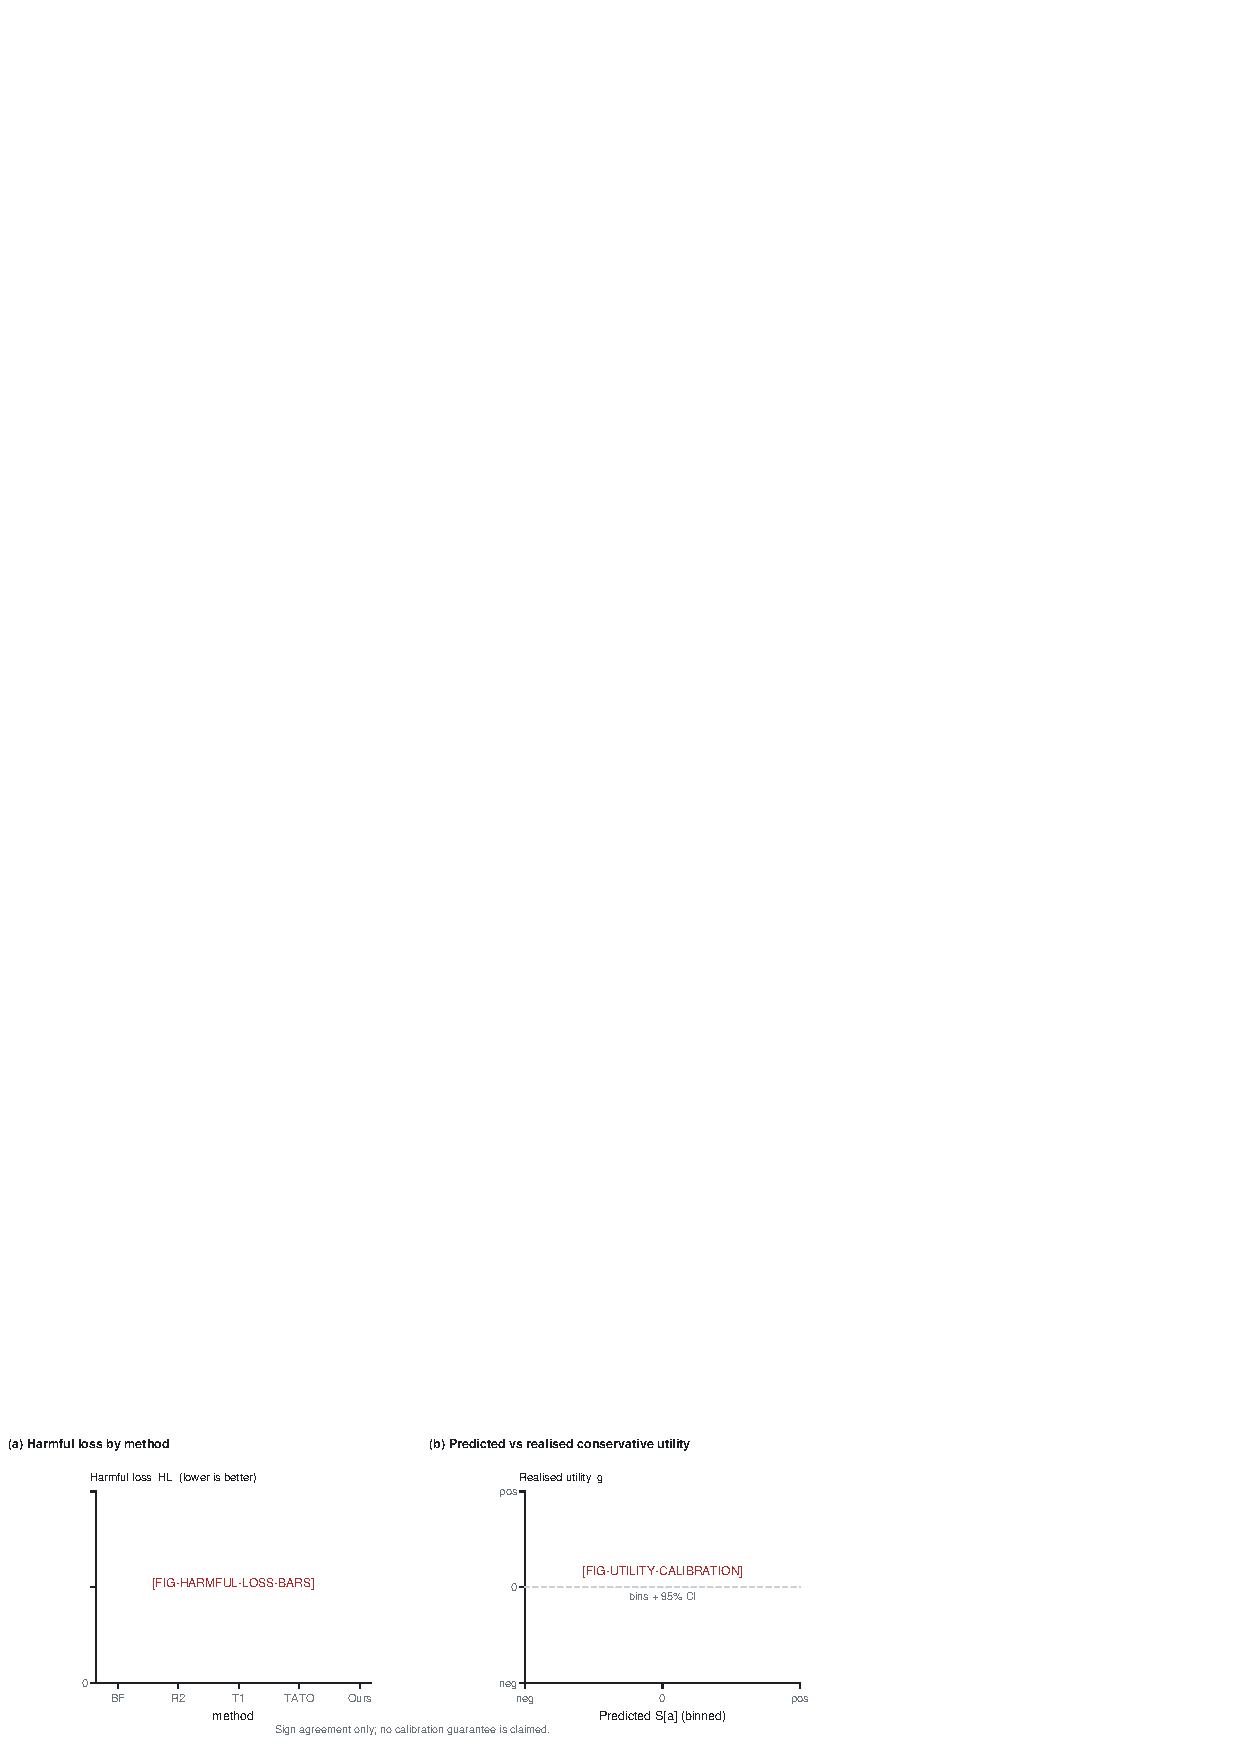
\includegraphics[width=0.84\textwidth]{figure/fig4_governance_diagnostics.pdf}
  \caption{\textbf{(a)}~Harmful loss by method. \textbf{(b)}~Realised utility against the
  binned conservative score with 95\% intervals. Panel~(b) is a sign agreement check, not a
  calibration claim.}
  \label{fig:governance}
\end{figure}

\section{Robustness Figure}
\label{app:robust-fig}
Figure~\ref{fig:robust} shows the severity trend summarised by Table~\ref{tab:robust}. Each
panel is a different frozen backbone; the axes are identical across panels so that the
panels can be compared directly.

\begin{figure}[h]
  \centering
  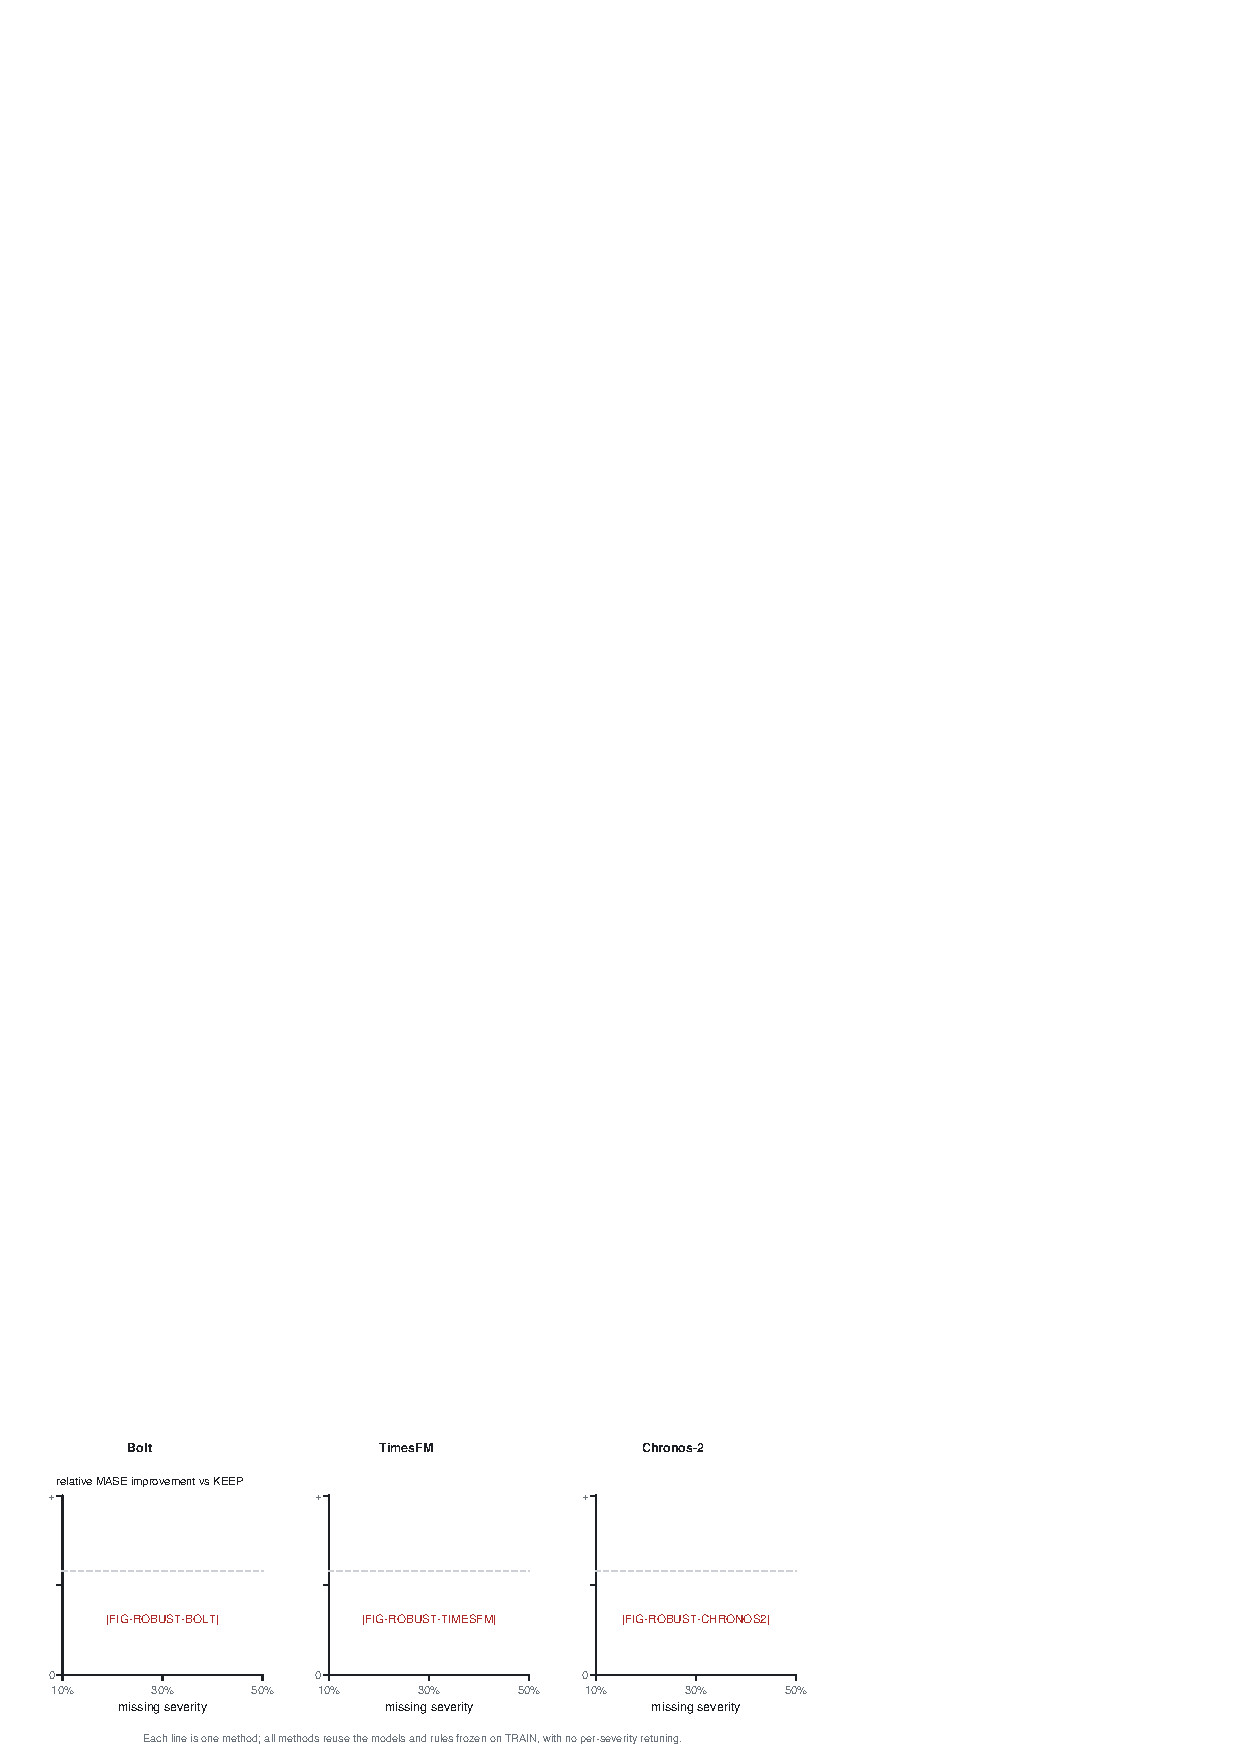
\includegraphics[width=0.86\textwidth]{figure/fig5_robustness_missingness.pdf}
  \caption{Relative MASE improvement over \textsc{Native Keep} as missingness severity
  increases, one line per method, one panel per frozen backbone. All methods reuse the
  models and rules frozen on TRAIN, with no per-severity retuning.}
  \label{fig:robust}
\end{figure}

\section{Replay Size}
\label{app:replaysize}
The replay bank is subsampled to $25\%$, $50\%$, and $100\%$ of its replay-fit support to
measure how much the method depends on the amount of historical evidence. This analysis is
not part of the main text and was not used to select any hyperparameter; the frozen
configuration is the one trained on the full bank. If performance at $25\%$ matches
performance at $100\%$, the honest reading is that the bank is already saturated at this
scale, not that the method is data-efficient in general.

\begin{table}[h]
  \caption{Replay-bank size ablation. The bank is subsampled by replay-fit parent, keeping
  every action and severity per retained parent, so the subsample changes the amount of
  history rather than its composition.}
  \label{tab:app-replaysize}
  \centering
  \small
  \setlength{\tabcolsep}{4pt}
  \begin{tabular}{lccccc}
    \toprule
    Bank fraction & MASE $\downarrow$ & Intervention Rate & HIR $\downarrow$ & Harmful Loss $\downarrow$ & Calls $\downarrow$ \\
    \midrule
    $25\%$  & \ph{RS25-MASE}  & \ph{RS25-IR}  & \ph{RS25-HIR}  & \ph{RS25-HL}  & \ph{RS25-CALLS} \\
    $50\%$  & \ph{RS50-MASE}  & \ph{RS50-IR}  & \ph{RS50-HIR}  & \ph{RS50-HL}  & \ph{RS50-CALLS} \\
    $100\%$ & \ph{RS100-MASE} & \ph{RS100-IR} & \ph{RS100-HIR} & \ph{RS100-HL} & \ph{RS100-CALLS} \\
    \bottomrule
  \end{tabular}
\end{table}

\section{$K$ and $\beta$ Sensitivity}
\label{app:ksens}
Table~\ref{tab:app-ksens} reports the full $3 \times 3$ grid over the neighbourhood size
$K \in \{8, 16, 32\}$ and the conservativeness level $\beta \in \{0, 1, 1.64\}$. The grid is
evaluated on the gate split only; the cell carried into the frozen configuration is marked.
The temperature is not part of the grid: it is fixed at
$\tau = \mathrm{median}(d_i) + \varepsilon$ precisely so that this search stays two-dimensional.

\begin{table}[h]
  \caption{$K$ and $\beta$ sensitivity on the gate split. Each cell reports MASE and the
  harmful intervention rate. The selected cell is marked with a dagger.}
  \label{tab:app-ksens}
  \centering
  \small
  \setlength{\tabcolsep}{4pt}
  \begin{tabular}{lccc}
    \toprule
    & $\beta = 0$ & $\beta = 1$ & $\beta = 1.64$ \\
    \midrule
    $K = 8$  & \ph{K8-B0}  & \ph{K8-B1}  & \ph{K8-B164} \\
    $K = 16$ & \ph{K16-B0} & \ph{K16-B1} & \ph{K16-B164} \\
    $K = 32$ & \ph{K32-B0} & \ph{K32-B1} & \ph{K32-B164} \\
    \bottomrule
  \end{tabular}
\end{table}

\section{Frozen-Model Call Accounting}
\label{app:calls}
Table~\ref{tab:app-calls} separates offline from online cost and separates successes from
failures. Failures and timeouts are never counted as successes and are never dropped from
the denominator; a request that fails to produce a forecast is reported as a failure, not
as a zero-cost success. The reference forecast always costs one call, and an executed
intervention costs a second one, so the call count is at most two per request.

\begin{table}[h]
  \caption{Frozen-model call accounting. Latency is reported per request and excludes cold
  start, which is reported on its own line; the offline replay-bank build is amortised and
  reported separately.}
  \label{tab:app-calls}
  \centering
  \small
  \setlength{\tabcolsep}{4pt}
\resizebox{\textwidth}{!}{\begin{tabular}{lccc}
    \toprule
    Outcome & Requests & Share & Frozen-model calls per request \\
    \midrule
    Abstained (reference forecast only) & \ph{CALLS-ABSTAIN-N} & \ph{CALLS-ABSTAIN-SHARE} & 1 \\
    Intervened (reference + one action) & \ph{CALLS-ACT-N}     & \ph{CALLS-ACT-SHARE}     & 2 \\
    Failed before any forecast          & \ph{CALLS-FAIL-N}    & \ph{CALLS-FAIL-SHARE}    & \ph{CALLS-FAIL-COST} \\
    Timed out after the reference       & \ph{CALLS-TIMEOUT-N} & \ph{CALLS-TIMEOUT-SHARE} & \ph{CALLS-TIMEOUT-COST} \\
    \midrule
    Offline replay-bank build (amortised) & --- & --- & \ph{CALLS-OFFLINE} \\
    Cold start (first request of a process) & \ph{CALLS-COLD-N} & --- & \ph{CALLS-COLD-LATENCY} \\
    \bottomrule
  \end{tabular}}
\end{table}

\section{Negative Result from the Preceding Development Cycle}
\label{app:r5}
An earlier configuration in this line of work attempted to improve intervention ranking by
projecting estimated gain vectors onto a convex feasible set, under a Frank--Wolfe
solver~\citep{boyd2004convex,jaggi2013revisiting}. The projection has a clean property ---
for an exact projection $z$ of a score vector $r$, one has
$\lVert z - g \rVert^2 \le \lVert r - g \rVert^2 - \lVert r - z \rVert^2$ for any feasible
true gain vector $g$ --- but that property controls the squared error of the whole vector
only. It does not guarantee per-coordinate improvement, does not preserve action ranking,
and does not imply a better MASE.

In that cycle the projection did reduce the squared error of the estimated gain vector
while failing to improve, and in one backbone degrading, the final forecasting metric.
Those measurements are recorded here because they motivate the design decision in
\S\ref{sec:method-gate}: continuous score calibration is insufficient for discrete
intervention selection, which is why \introact{} scores actions with an explicitly
conservative mean-minus-uncertainty quantity and abstains rather than refining a score.
The recorded measurements belong to the preceding protocol (a small development split of
26 parents with 156 correlated variants, two backbones, and a different action budget
accounting). They are reproduced below verbatim from the frozen ledger and must not be
compared numerically with any table in this paper.

\begin{table}[h]
  \caption{Preceding-cycle measurements, retained as a negative result. Different protocol
  from the present paper: 26 development parents, 156 correlated variants, different
  budget accounting. Values are quoted from the frozen ledger and are \emph{not}
  comparable with Tables~\ref{tab:main}--\ref{tab:robust}.}
  \label{tab:r5negative}
  \centering
  \small
  \begin{tabular}{llcc}
    \toprule
    Backbone & Configuration & MASE $\downarrow$ & Note \\
    \midrule
    Bolt     & Native KEEP (no governance)   & 1.258454 & reference \\
    Bolt     & Free reference policy         & 1.152415 & equals the full candidate \\
    Bolt     & Projection candidate          & 1.152415 & no gain over the free reference \\
    TimesFM  & Native KEEP (no governance)   & 1.139837 & reference \\
    TimesFM  & Strong simple TRAIN control   & 1.069398 & strongest simple rule \\
    TimesFM  & Projection candidate          & 1.074244 & worse than the simple control \\
    \bottomrule
  \end{tabular}
\end{table}

Two consequences of that cycle are load-bearing for the present paper. First, the strongest
simple selector available at the time (\textbf{R2-CART} in the present terminology) was
competitive with, and on one backbone better than, the more elaborate candidate; that is
why R2-CART is carried forward as a mandatory control in every main-text table. Second,
reducing estimation error on a continuous score was not sufficient to improve discrete
selection; that is why the conservative gate in \S\ref{sec:method-gate} is evaluated
directly on harmful intervention rate and harmful loss, not only on MASE.

\section{Complete Input Contract}
\label{app:complete}
Under a complete and valid input, \introact{} must return \textsc{Keep}. No forecasting
improvement is claimed in this regime; the purpose of this appendix is to document the
governance contract rather than to report a result. Table~\ref{tab:app-complete} lists the
regimes and the required behaviour in each.

\begin{table}[h]
  \caption{Governance contract by input regime. The complete-input rows are contract
  statements, not accuracy results: the expected behaviour is a no-op, and a non-no-op
  there would be a defect rather than an improvement.}
  \label{tab:app-complete}
  \centering
  \small
  \setlength{\tabcolsep}{4pt}
\resizebox{\textwidth}{!}{\begin{tabular}{lll}
    \toprule
    Input regime & Required behaviour & Claim \\
    \midrule
    Complete and valid input            & return \textsc{Keep} and the reference forecast & no-op contract, no accuracy claim \\
    Complete input, malformed request   & reject with an explicit status & no claim \\
    Unsupported action requested        & reject the action, keep the catalog closed & no claim \\
    Incomplete input, no strong evidence& abstain, return the reference forecast & abstention is a valid outcome \\
    Incomplete input, strong evidence   & execute exactly one action and return its forecast & evaluated in \S\ref{sec:exp-main} \\
    \bottomrule
  \end{tabular}}
\end{table}

\section{Finance Case Study}
\label{app:finance}
The two finance parents currently available are reported as a case study only. We do not
claim financial generalisation. Results are reported separately for the complete-observed
condition and for controlled deletion, and verified natural missingness is reported only
if it exists; where it does not, that is stated rather than substituted with synthetic
gaps. QLIKE is reported here and nowhere else. The finance series contain real jumps, such
as market closures; these are not smoothed and are not filled as if they were missing
observations.

\begin{table}[h]
  \caption{Finance case study. The complete-observed rows are the no-op check; the
  controlled-deletion rows carry the only quantitative comparison. Natural missingness is
  listed only where it has been verified.}
  \label{tab:app-finance}
  \centering
  \small
  \setlength{\tabcolsep}{4pt}
\resizebox{\textwidth}{!}{\begin{tabular}{llcccc}
    \toprule
    Parent & Condition & MASE $\downarrow$ & QLIKE $\downarrow$ & Harmful Rate & Note \\
    \midrule
    \ph{FIN-P1} & complete observed     & \ph{FIN-P1-COMP-MASE} & \ph{FIN-P1-COMP-QLIKE} & --- & no-op check \\
    \ph{FIN-P1} & controlled deletion   & \ph{FIN-P1-DEL-MASE}  & \ph{FIN-P1-DEL-QLIKE}  & \ph{FIN-P1-HIR} & \ph{FIN-P1-NOTE} \\
    \ph{FIN-P2} & complete observed     & \ph{FIN-P2-COMP-MASE} & \ph{FIN-P2-COMP-QLIKE} & --- & no-op check \\
    \ph{FIN-P2} & controlled deletion   & \ph{FIN-P2-DEL-MASE}  & \ph{FIN-P2-DEL-QLIKE}  & \ph{FIN-P2-HIR} & \ph{FIN-P2-NOTE} \\
    \midrule
    \multicolumn{6}{l}{\footnotesize Verified natural missingness: \ph{FIN-NATURAL-STATUS}} \\
    \bottomrule
  \end{tabular}}
\end{table}

\section{Ten Mask Seeds}
\label{app:seeds}
The main experiment uses one deterministic mask per parent. This appendix reruns a
pre-registered representative protocol with ten additional mask seeds to show that the
conclusions are stable with respect to mask realisation. The ten seeds are \emph{not}
treated as ten independent parents and are never used for significance testing: the
statistical unit remains the parent, and the seeds are read as a stability check on the
same parent set.

\begin{table}[h]
  \caption{Mask-seed stability. Each row is one additional mask realisation on the
  pre-registered representative parent subset. Spread across seeds is a stability
  diagnostic, not an additional sample of parents.}
  \label{tab:app-seeds}
  \centering
  \small
  \setlength{\tabcolsep}{4pt}
  \begin{tabular}{lccc}
    \toprule
    Mask seed & MASE $\downarrow$ & $\Delta$ vs \textsc{Keep} $\uparrow$ & Intervention Rate \\
    \midrule
    \ph{SEED-1}  & \ph{SEED1-MASE}  & \ph{SEED1-DELTA}  & \ph{SEED1-IR} \\
    \ph{SEED-2}  & \ph{SEED2-MASE}  & \ph{SEED2-DELTA}  & \ph{SEED2-IR} \\
    \ph{SEED-3}  & \ph{SEED3-MASE}  & \ph{SEED3-DELTA}  & \ph{SEED3-IR} \\
    \ph{SEED-4}  & \ph{SEED4-MASE}  & \ph{SEED4-DELTA}  & \ph{SEED4-IR} \\
    \ph{SEED-5}  & \ph{SEED5-MASE}  & \ph{SEED5-DELTA}  & \ph{SEED5-IR} \\
    \ph{SEED-6}  & \ph{SEED6-MASE}  & \ph{SEED6-DELTA}  & \ph{SEED6-IR} \\
    \ph{SEED-7}  & \ph{SEED7-MASE}  & \ph{SEED7-DELTA}  & \ph{SEED7-IR} \\
    \ph{SEED-8}  & \ph{SEED8-MASE}  & \ph{SEED8-DELTA}  & \ph{SEED8-IR} \\
    \ph{SEED-9}  & \ph{SEED9-MASE}  & \ph{SEED9-DELTA}  & \ph{SEED9-IR} \\
    \ph{SEED-10} & \ph{SEED10-MASE} & \ph{SEED10-DELTA} & \ph{SEED10-IR} \\
    \midrule
    Spread (max $-$ min) & \ph{SEED-SPREAD} & --- & \ph{SEED-IR-SPREAD} \\
    \bottomrule
  \end{tabular}
\end{table}

\section{Additional Horizons}
\label{app:horizons}
Longer horizons are reported here and are excluded from the main text, so that the main
comparison stays on the two horizons that every baseline can serve. These horizons are
reported for completeness; a conclusion that only holds at a longer horizon is not
presented as a main claim.

\begin{table}[h]
  \caption{Additional horizons beyond the two main ones, source-macro averaged, $10\%$
  severity. Reported for completeness and excluded from all main-text ranks.}
  \label{tab:app-horizons}
  \centering
  \small
  \setlength{\tabcolsep}{4pt}
\resizebox{\textwidth}{!}{\begin{tabular}{lccccc}
    \toprule
    Horizon & Method & MASE $\downarrow$ & MSE $\downarrow$ & MAE $\downarrow$ & RMSSE $\downarrow$ \\
    \midrule
    \ph{HX1} & \introact{} & \ph{HX1-OURS-MASE} & \ph{HX1-OURS-MSE} & \ph{HX1-OURS-MAE} & \ph{HX1-OURS-RMSSE} \\
    \ph{HX1} & \textsc{Native Keep} & \ph{HX1-KEEP-MASE} & \ph{HX1-KEEP-MSE} & \ph{HX1-KEEP-MAE} & \ph{HX1-KEEP-RMSSE} \\
    \ph{HX2} & \introact{} & \ph{HX2-OURS-MASE} & \ph{HX2-OURS-MSE} & \ph{HX2-OURS-MAE} & \ph{HX2-OURS-RMSSE} \\
    \ph{HX2} & \textsc{Native Keep} & \ph{HX2-KEEP-MASE} & \ph{HX2-KEEP-MSE} & \ph{HX2-KEEP-MAE} & \ph{HX2-KEEP-RMSSE} \\
    \bottomrule
  \end{tabular}}
\end{table}

\section{Reproducibility Details}
\label{app:reprodetails}
Each record in the result files contains: source, parent, origin, horizon, pattern,
severity, mask hash, backbone, backbone revision, method, action, input hash, prediction
hash, forecast, target reference id, MASE, MSE, MAE, RMSSE, reconstruction MSE where
applicable, runtime components, failure, fallback, code SHA, and resolved configuration.
Results are written to the logical result groups listed in Table~\ref{tab:app-groups}, each
in CSV, JSON, and Markdown form, with raw predictions retained alongside the aggregates.

\begin{table}[h]
  \caption{Result groups written by the pipeline. Every number in the main text and in the
  appendices is generated from one of these groups; nothing is transcribed by hand.}
  \label{tab:app-groups}
  \centering
  \small
  \setlength{\tabcolsep}{4pt}
\resizebox{\textwidth}{!}{\begin{tabular}{lll}
    \toprule
    Result group & Contents & Consumed by \\
    \midrule
    \texttt{v44\_protocol}       & frozen protocol, source manifests, split bounds & Appendix~\ref{app:protocol} \\
    \texttt{v44\_replay\_bank}   & replay records $(z_i, a, g_{i,a})$ with input and prediction hashes & \S\ref{sec:method-replay} \\
    \texttt{v44\_baselines}      & baseline training runs, resolved hyperparameters, checkpoints & \S\ref{sec:exp-main} \\
    \texttt{v44\_train\_eval}    & TRAIN-eval acceptance check before freezing & Appendix~\ref{app:splits} \\
    \texttt{v44\_main\_results}  & main matrix rows, all methods, all cells & Tables~\ref{tab:main}, \ref{tab:app-src-bolt}--\ref{tab:app-src-ch2} \\
    \texttt{v44\_ablation}       & the six ablation variants & Table~\ref{tab:ablation} \\
    \texttt{v44\_robustness}     & severity, pattern, and mask-seed sweeps & Tables~\ref{tab:robust}, \ref{tab:app-sev10}--\ref{tab:app-sev50}, \ref{tab:app-seeds} \\
    \texttt{v44\_cost\_audit}    & call counts, latency, failures, timeouts & Table~\ref{tab:efficiency}, Appendix~\ref{app:calls} \\
    \bottomrule
  \end{tabular}}
\end{table}

The protocol is frozen before the main experiment and identified by commit hash. Any
change to the action catalog, the missingness protocol, the mask derivation rule, the split
boundaries, the state feature list, or the failure policy invalidates the freeze and
requires a new configuration identifier. Calibration and test labels are not read during
development, and no result in this paper is selected on them.

\end{document}
